%% This template can be used to write a paper for
%% Computer Physics Communications using LaTeX.
%% For authors who want to write a computer program description,
%% an example Program Summary is included that only has to be
%% completed and which will give the correct layout in the
%% preprint and the journal.
%% The `elsarticle' style is used and more information on this style
%% can be found at
%% http://www.elsevier.com/wps/find/authorsview.authors/elsarticle.
%%
%%
\documentclass[preprint,12pt]{elsarticle}

%% Use the option review to obtain double line spacing
%% \documentclass[preprint,review,12pt]{elsarticle}

%% Use the options 1p,twocolumn; 3p; 3p,twocolumn; 5p; or 5p,twocolumn
%% for a journal layout:
%% \documentclass[final,1p,times]{elsarticle}
%% \documentclass[final,1p,times,twocolumn]{elsarticle}
%% \documentclass[final,3p,times]{elsarticle}
%% \documentclass[final,3p,times,twocolumn]{elsarticle}
%% \documentclass[final,5p,times]{elsarticle}
%% \documentclass[final,5p,times,twocolumn]{elsarticle}

%% if you use PostScript figures in your article
%% use the graphics package for simple commands
%% \usepackage{graphics}
%% or use the graphicx package for more complicated commands
\usepackage{graphicx}
%% or use the epsfig package if you prefer to use the old commands
%% \usepackage{epsfig}

%% The amssymb package provides various useful mathematical symbols
\usepackage{amssymb}
%% The amsthm package provides extended theorem environments
%% \usepackage{amsthm}

%% The lineno packages adds line numbers. Start line numbering with
%% \begin{linenumbers}, end it with \end{linenumbers}. Or switch it on
%% for the whole article with \linenumbers after \end{frontmatter}.
%% \usepackage{lineno}

% jons ::: my own packages ::: jons
\usepackage{siunitx}
\usepackage{amsmath}
\usepackage{cancel}
\usepackage{hyperref}

\def\eqn#1{Eqn.~(\ref{eqn:#1})}

% \intercal for transpose, \mathbb{R} reals, \mathbb{C} complex numbers
% \usepackage{amssymb} (already provided by template)
% \def\realnumbers{\rm I\!R} % does not generalize to complex numbers...
\def\naturals{\mathbb{N}}
\def\naturalsWithZero{\mathbb{N}_0}
\def\integers{\mathbb{Z}}
\def\realnumbers{\mathbb{R}}
\def\complexnumbers{\mathbb{C}}

% \mathfrak{Re}, \mathfrak{Im}
% \usepackage[frak=esstix]{mathalpha} % on some other systems...
\usepackage[frak=esstix]{mathalfa}
\def\realpart{\mathfrak{Re}}
\def\imagpart{\mathfrak{Im}}

% end ::: my own packages ::: end




%% natbib.sty is loaded by default. However, natbib options can be
%% provided with \biboptions{...} command. Following options are
%% valid:

%%   round  -  round parentheses are used (default)
%%   square -  square brackets are used   [option]
%%   curly  -  curly braces are used      {option}
%%   angle  -  angle brackets are used    <option>
%%   semicolon  -  multiple citations separated by semi-colon
%%   colon  - same as semicolon, an earlier confusion
%%   comma  -  separated by comma
%%   numbers-  selects numerical citations
%%   super  -  numerical citations as superscripts
%%   sort   -  sorts multiple citations according to order in ref. list
%%   sort&compress   -  like sort, but also compresses numerical citations
%%   compress - compresses without sorting
%%
%% \biboptions{comma,round}

% \biboptions{}

%% This list environment is used for the references in the
%% Program Summary
%%
\newcounter{bla}
\newenvironment{refnummer}{%
\list{[\arabic{bla}]}%
{\usecounter{bla}%
 \setlength{\itemindent}{0pt}%
 \setlength{\topsep}{0pt}%
 \setlength{\itemsep}{0pt}%
 \setlength{\labelsep}{2pt}%
 \setlength{\listparindent}{0pt}%
 \settowidth{\labelwidth}{[9]}%
 \setlength{\leftmargin}{\labelwidth}%
 \addtolength{\leftmargin}{\labelsep}%
 \setlength{\rightmargin}{0pt}}}
 {\endlist}

\journal{Computer Physics Communications}

\begin{document}

\begin{frontmatter}

%% Title, authors and addresses

%% use the tnoteref command within \title for footnotes;
%% use the tnotetext command for the associated footnote;
%% use the fnref command within \author or \address for footnotes;
%% use the fntext command for the associated footnote;
%% use the corref command within \author for corresponding author footnotes;
%% use the cortext command for the associated footnote;
%% use the ead command for the email address,
%% and the form \ead[url] for the home page:
%%
%% \title{Title\tnoteref{label1}}
%% \tnotetext[label1]{}
%% \author{Name\corref{cor1}\fnref{label2}}
%% \ead{email address}
%% \ead[url]{home page}
%% \fntext[label2]{}
%% \cortext[cor1]{}
%% \address{Address\fnref{label3}}
%% \fntext[label3]{}

\title{Accurate Biot-Savart Routines with Correct Asymptotic Behaviour}

%% use optional labels to link authors explicitly to addresses:
%% \author[label1,label2]{<author name>}
%% \address[label1]{<address>}
%% \address[label2]{<address>}

\author[a]{Jonathan Schilling\corref{author}}
\author[a]{Jakob Svensson}
\author[a]{Joachim Geiger}
% \author[a,b]{Second Author}
% \author[b]{Third Author}

\cortext[author] {Corresponding author.\\\textit{E-mail address:} jonathan.schilling@ipp.mpg.de}
\address[a]{Max-Planck-Institute for Plasma Physics, Wendelsteinstrasse 1, 17489 Greifswald, Germany}
% \address[b]{Second Address}

\begin{abstract}
A set of routines to compute the magnetic vector potential and magnetic field of two types of current carriers is presented.
The (infinitely thin) current carrier types are a straight wire segment and a circular wire loop.
The routines are highly accurate and exhibit the correct asymptotic behaviour far away from and close to the current carrier.
A suitable global set of test points is introduced and the methods presented in this work
are tested against results obtained using arbitrary-precision arithmetic on all test points.
The results are accurate to approximately 16 decimal digits of precision when computed using 64 bit floating point arithmetic,
with few exceptions where accuracy drops to 12 digits.
These primitive types can be used to make up more complex current carrier arrangements,
such as a current along a polygon (by means of defining straight wire segments from point to point of the polygon)
and a multi-winding coil with circular cross-section (by positioning circular wire loops at appropriate positions in the coils cross-section).
Reference data is provided along with the code to compute it
for testing the reader's routines against this work.
\end{abstract}

\begin{keyword}
%% keywords here, in the form: keyword \sep keyword
magnetostatics; Biot-Savart; straight wire segment; circular wire loop; magnetic vector potential; magnetic field
\end{keyword}

\end{frontmatter}

%%
%% Start line numbering here if you want
%%
% \linenumbers

% All CPiP articles must contain the following
% PROGRAM SUMMARY.

{\bf PROGRAM SUMMARY}

\begin{small}
\noindent
{\em Program Title:} Accurate Biot-Savart Routines with Correct Asymptotic Behaviour \\
{\em CPC Library link to program files:} (to be added by Technical Editor) \\
{\em Developer's repository link:} https://github.com/jonathanschilling/abscab \\
{\em Code Ocean capsule:} (to be added by Technical Editor)\\
{\em Licensing provisions(please choose one):} Apache-2.0 \\
{\em Programming language:} C                                  \\
{\em Supplementary material:}                                 \\
  % Fill in if necessary, otherwise leave out.
{\em Nature of problem(approx. 50-250 words):}\\
  %Describe the nature of the problem here. \\
{\em Solution method(approx. 50-250 words):}\\
  %Describe the method solution here.
{\em Additional comments including restrictions and unusual features (approx. 50-250 words):}\\
  %Provide any additional comments here.
   \\

\begin{thebibliography}{0}
\bibitem{1}Reference 1         % This list should only contain those items referenced in the
\bibitem{2}Reference 2         % Program Summary section.
\bibitem{3}Reference 3         % Type references in text as [1], [2], etc.
                               % This list is different from the bibliography at the end of the Long Write-Up.
\end{thebibliography}
\end{small}


%% main text
\section{Introduction}
\label{sec:introduction}
A common task in computational physics is to compute the magnetic field and magnetic vector potential
originating from current-carrying wire arrangements in the form of coils and cables.
These current carriers can be approximated for computational simplicity as infinitely thin filaments
following the center lines of the real current carrier.
A current carrier path specified by a list of points along the path
can be modeled as a set of straight wire segments from point to point along the polygon describing the current carrier geometry.
Closed circular wire loops appear as well in practise and can be chosen to model, e.g.,
individual windings in a circular coil.
Computational methods are thus needed to compute the magnetic field and the magnetic vector potential
of a single straight wire segment or a single circular wire loop
in order to model more complex current carrier arrangements
by superposition of the current carrier primitives.
Analytical expressions are derived in this work to accurately compute
the magnetic field and the magnetic vector potential of a straight wire segment
and a circular wire loop. The expressions consist of several special cases,
which are switched between depending on the location of the evaluation location
in the coordinate system of the current carrier primitive.
This approach allows to select the most accurate formulation
for a given evaluation location and make explicit use of simplications
in certain special cases for the sake of simplicity, speed and accuracy.
Particular attention was paid to make sure that the expressions presented in this work
obey the correct asymptotic behavior for evaluation locations
far away from and close to the current carriers.
For most test cases, the full relative accuracy of the floating point
arithmetic chosen for implementation is retained throughout the computations
(16 digits of precision in the \texttt{float64} implementation),
with few exceptions where accuracy drops by up to 2 digits of precision
(in the \texttt{float64} case).
The provided implementations have not been optimized for speed.

The magnetic field is denoted by $\mathbf{H}$ and
the magnetic flux density $\mathbf{B}$ is then given by $\mathbf{B} = \mu_0 \mu_\mathrm{r} \mathbf{H}$,
where $\mu_0$ is the vacuum magnetic permeability
and $\mu_r$ is the relative permeability, taking material properties into account.
In the field of plasma physics generally and in this work in particular,
these two terms are frequently used synonymously
due to the vanishing magnetic susceptibility $|\chi| \ll 1$ of the plasma,
leading to $\mu_r = 1+\chi \approx 1$.
This is equivalent to considering only vacuum magnetic fields.
Then, magnetic field and magnetic flux density only differ by a factor of $\mu_0$.

\FloatBarrier
\section{Methods}
\label{sec:methods}
In this section, accurate methods used to compute the magnetic vector potential~$\mathbf{A}$ and the magnetic field~$\mathbf{B}$
of a straight wire segment and a circular wire loop are presented.
Furthermore, methods to evaluate the magnetostatic quantities in global coordinates are provided.
Particular attention was paid to ensure that the expressions presented in this work
obey the correct asymptotic behavior for evaluation locations
far away from and close to the current carriers.
For most test cases, the full relative accuracy of the floating point
arithmetic chosen for implementation is retained throughout the computations
(16 digits of precision in the IEEE-754 \texttt{binary64}~\cite{ieee754} implementation).
There are a few exceptions where accuracy drops by up to 3 digits of precision
(in the \texttt{binary64} case).
The section concludes with a description of the verification procedure
employed to benchmark these methods.

\FloatBarrier
\subsection{Straight Wire Segment}
\label{sec:methods_sws}
The basic geometry of a single wire segment is shown in Fig.~\ref{fig:straightWireSegment}.
A cylindrical coordinate system~$(\rho, \varphi,z)$ is aligned with the wire segment~(red line),
such that the wire is aligned with the $z$-axis and starts at the origin.
A current $I$ flows along the wire segment of length~$L$ in positive~$z$ direction~(red arrow).
The evaluation point is specified by~$\mathbf{x} = (\rho, \varphi=0, z)$.
$R_\mathrm{i}$ ($R_\mathrm{f}$) denotes the distance from the start (end) of the wire segment to~$\mathbf{x}$.
The angles $\alpha$ and $\beta$ are used in the formulas below.
\begin{figure}[htbp]
 \centering
 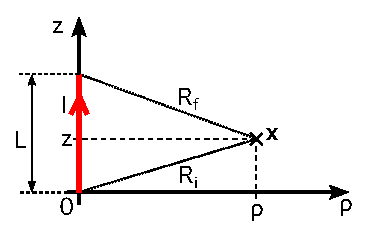
\includegraphics[width=8cm]{img/straightWireSegment.eps}
%  \includegraphics[width=8cm]{img/figure_1.eps}
 \caption{Geometry of a single wire segment (red line) and the associated cylindrical coordinate system.
          The magnetostatic quantities are to be evaluated at a location $\mathbf{x}$.
          After Fig.~1 in Ref.~\cite{hanson_hirshman_2002}.}
 \label{fig:straightWireSegment}
\end{figure}

\subsubsection{Magnetic Vector Potential}
\label{sec:methods_sws_vecpot}
The magnetic vector potential of a straight wire segment
only has component~$A_z$ parallel to the wire:
\begin{equation}
 \mathbf{A} = A_z \hat{\mathbf{e}}_z
\end{equation}
where~$\hat{\mathbf{e}}_z$ is the unit vector in direction $z$.
It is given by~\cite{hanson_hirshman_2002}:
\begin{equation}
  A_z(\rho, z) = \frac{\mu_0 I}{4 \pi} \ln \left( \frac{1 + \epsilon}{1 - \epsilon} \right)
\end{equation}
with
\begin{align}
  \epsilon =&\, \frac{L}{R_\mathrm{i} + R_\mathrm{f}} \\
       R_\mathrm{i} =&\, \sqrt{\rho^2 + z^2} \\
       R_\mathrm{f} =&\, \sqrt{\rho^2 + (1 - z)^2} \, .
\end{align}
In this work normalized coordinates~$\rho' = \rho/L$ and~$z' = z/L$ are used.
This leads to the following expressions
for~$r_\mathrm{i} = R_\mathrm{i}/L$ and~$r_\mathrm{f} = R_\mathrm{f}/L$:
\begin{align}
  r_\mathrm{i} =&\, \sqrt{{\rho'}^2 +      {z'}^2 }       \label{eqn:r_i_default} \\
  r_\mathrm{f} =&\, \sqrt{{\rho'}^2 + (1 - {z'})^2}       \label{eqn:r_f_default} \\
  \Rightarrow
  \epsilon     =&\, \frac{1}{r_\mathrm{i} + r_\mathrm{f}} \label{eqn:eps_default}\, .
\end{align}
For locations on the conductor, $\epsilon = 1$ holds.
The magnetostatic quantites are not defined for evaluation locations on the conductor,
which implies $\epsilon < 1$ for valid evaluation locations.
The value of $\epsilon$ only depends on the sum $r_\mathrm{i} + r_\mathrm{f}$,
which implies that contours of constant $\epsilon$ are ellipses with focii at the ends of the wire segment.
This is similar to the Gardener's construction method for ellipses~\cite{dawson_2021}.
The elliptical contours of constant $\epsilon$ are illustrated in Fig.~\ref{fig:epsilon_contours}.
The contours approach a circular shape far away from the wire segment.
\begin{figure}[htbp]
 \centering
 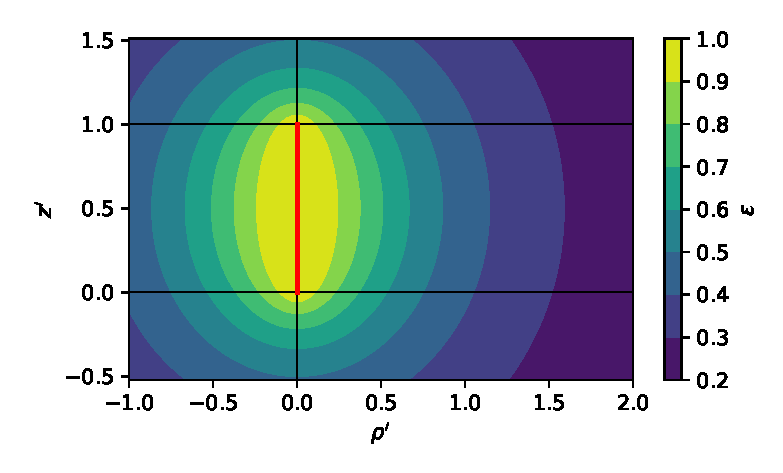
\includegraphics{img/epsilon_contours.eps}
%  \includegraphics{img/figure_2.eps}
 \caption{Contours of constant $\epsilon$ as computed from \eqn{eps_default}.
          The straight wire segment is located along the red line.}
 \label{fig:epsilon_contours}
\end{figure}
A common prefactor depending on the current~$I$ and~$\mu_0$ is split off:
\begin{equation}
  A_z(\rho', z') = \frac{\mu_0 I}{2 \pi} \tilde{A}_z (\rho', z')
\end{equation}
with
\begin{equation}
  \tilde{A}_z (\rho', z')
  = \frac{1}{2} \ln \left( \frac{1 + \epsilon}{1 - \epsilon} \right)
  = \textrm{atanh} (\epsilon) \, . \label{eqn:A_z_tilde}
\end{equation}
The rest of this section is dedicated to the accurate computation of $\tilde{A}_z (\rho', z')$.
One of several formulations is chosen depending on the evaluation location~$(\rho', z')$:
\begin{equation}
  \tilde{A}_z (\rho', z') =
  \begin{cases}
    \textrm{undefined}                   &:\, \rho' = 0; 0 \leq z' \leq 1 \\
    \tilde{A}_\mathrm{z,ax}  (z')        &:\, \rho' = 0; z' < 0 \textrm{ or } z' > 1  \\
    \tilde{A}_\mathrm{z,rad} (\rho')     &:\, \rho' > 0; z' \in \{0, 1\} \\
    \tilde{A}_\mathrm{z,f}   (\rho', z') &:\, (\rho' \geq 1 \textrm{ and } z' \,\cancel{\in}\, \{0, 1\}) \textrm{ or } \\
                ~                        &~\,\, (\rho' > 0; z' \leq -1 \textrm{ or } z' > 2) \\
    \tilde{A}_\mathrm{z,n}   (\rho', z') &:\, \textrm{elsewhere.}
  \end{cases} \label{eqn:sws_A_z_switchover}
\end{equation}
The domain decomposition for the accurate computation of $\tilde{A}_z$
formulated in \eqn{sws_A_z_switchover} is illustrated in Fig.~\ref{fig:sws_regions}(a).
For the case~$\rho'=0$, the following formulation is used:
\begin{equation}
  \tilde{A}_\mathrm{z,ax} (z') =
  \begin{cases}
    \textrm{undefined}             &:\, 0 \leq z' \leq 1 \\
    \tilde{A}_\mathrm{z,ax,f} (z') &:\, z' < -1 \textrm{ or } z' \geq 2 \\
    \tilde{A}_\mathrm{z,ax,n} (z') &:\, -1 \leq z' < 0 \textrm{ or } 1 < z' < 2
  \end{cases}
\end{equation}
with
\begin{equation}
  \tilde{A}_\mathrm{z,ax,f} (z') = \textrm{atanh}\left( \frac{1}{|z'| + |1 - z'|} \right) \label{eqn:sws_A_z_ax_f}
\end{equation}
(derived in \eqn{sws_A_z_ax_f_derivation})
and
\begin{equation}
  \tilde{A}_\mathrm{z,ax,n} (z') = \frac{1}{2} \frac{z'}{|z'|} \ln \left(\frac{z'}{z' - 1}\right) \label{eqn:sws_A_z_ax_n} \, ,
\end{equation}
which is derived in \eqn{sws_A_z_ax_n_derivation}.
The cases with $z'=0$ or $z'=1$ are evaluated using the following expression:
\begin{equation}
  \tilde{A}_\mathrm{z,rad} (\rho') =
  \begin{cases}
    \textrm{undefined}                 &:\, \rho' = 0 \\
    \tilde{A}_\mathrm{z,rad,f} (\rho') &:\, \rho' > 1 \\
    \tilde{A}_\mathrm{z,rad,n} (\rho') &:\, 0 < \rho' \leq 1
  \end{cases}
\end{equation}
with
\begin{equation}
  \tilde{A}_\mathrm{z,rad,f} (\rho') = \textrm{atanh}\left( \frac{1}{\rho' + \sqrt{{\rho'}^2 + 1}} \right) \label{eqn:sws_A_z_rad_f}
\end{equation}
(derived in \eqn{sws_A_z_rad_f_derivation})
and
\begin{equation}
  \tilde{A}_\mathrm{z,rad,n} (\rho') = \frac{1}{2} \ln \left(\frac{\rho' c + 1 + c}{\rho' c + 2 s^2 }\right) \label{eqn:sws_A_z_rad_n}
\end{equation}
where
\begin{align}
  c =&\, \frac{1}{\sqrt{{\rho'}^2 + 1}} \\
  s =&\, \sin(\arctan(\rho')/2) \, .
\end{align}
The derivation for this formulation can be found in \eqn{sws_A_z_rad_n_derivation}.
The case of~$\tilde{A}_\mathrm{z,f}(\rho', z')$ is the straight-forward implementation of:
\begin{equation}
  \tilde{A}_\mathrm{z,f}(\rho', z') = \textrm{atanh} (\epsilon)
\end{equation}
with~$r_\mathrm{i}$, $r_\mathrm{f}$ and~$\epsilon$ from~\eqn{r_i_default}, \eqn{r_f_default} and~\eqn{eps_default}, respectively.
For all other permitted locations, the following evaluation is used:
\begin{equation}
  \tilde{A}_\mathrm{z,n} (\rho', z') = \frac{1}{2} \left[ \ln\left(n + 1 \right) - \ln \left( n \right)  \right] \label{eqn:sws_A_z_n}
\end{equation}
with
\begin{align}
  n                       =&\, r_\mathrm{i} \sin^2(\alpha/2) + r_\mathrm{f} \sin^2(\beta/2) \\
  \alpha =&\, \texttt{atan2}(\rho', z')   \label{eqn:sws_alpha} \\
  \beta  =&\, \texttt{atan2}(\rho', 1-z') \label{eqn:sws_beta}
\end{align}
and~$r_\mathrm{i}$, $r_\mathrm{f}$ from~\eqn{r_i_default}, \eqn{r_f_default}, respectively.
Trigonometric functions are used here since they offer increased numerical robustness
for the evaluation locations under consideration in this case.
The derivation for this formulation is found in the appendix around \eqn{sws_A_z_n_derivation}.

\subsubsection{Magnetic Field}
\label{sec:methods_sws_magfld}
The magnetic field of a straight wire segment
is given by the law of Biot and Savart as follows~\cite{hanson_hirshman_2002}:
\begin{equation}
 \mathbf{B}
 = \frac{\mu_0 I}{4 \pi}
   \hat{\mathbf{e}}_z \times \mathbf{R}_\mathrm{i}
   \frac{2 L (R_\mathrm{i} + R_\mathrm{f})}{R_\mathrm{i} R_\mathrm{f}} \frac{1}{\left(R_\mathrm{i} + R_\mathrm{f}\right)^2 - L^2} \, . \label{eqn:sws_B_phi}
\end{equation}
The vector~$\mathbf{R}_\mathrm{i}$ has components in directions parallel~($z$) and perpendicular~($\rho$) to the wire segment:
\begin{equation}
 \mathbf{R}_\mathrm{i}
 = z \,\hat{\mathbf{e}}_z + \rho \,\hat{\mathbf{e}}_\rho \label{eqn:R_i_vec}
\end{equation}
where $\rho$ and $z$ are cylindrical coordinates in the coordinate system aligned with the wire segment.
The vector-valued term in~\eqn{sws_B_phi} is reformulated as follows by inserting \eqn{R_i_vec}:
\begin{align}
 \hat{\mathbf{e}}_z \times \mathbf{R}_\mathrm{i}
 =&\, \hat{\mathbf{e}}_z \times \left( z \,\hat{\mathbf{e}}_z + \rho \,\hat{\mathbf{e}}_\rho \right) \nonumber \\
 =&\,      z \underbrace{\hat{\mathbf{e}}_z \times \hat{\mathbf{e}}_z}_{=0}
      + \rho \underbrace{\hat{\mathbf{e}}_z \times \hat{\mathbf{e}}_\rho}_{=\hat{\mathbf{e}}_\varphi}
 = \rho \,\hat{\mathbf{e}}_\varphi \, .
\end{align}
It follows that the magnetic field of a straight wire segment only has a component~$B_\varphi$ in tangential~($\varphi$) direction:
\begin{equation}
 \mathbf{B} = B_\varphi \hat{\mathbf{e}}_\varphi
\end{equation}
with
\begin{equation}
 B_\varphi (\rho, z)
 = \frac{\mu_0 I}{4 \pi}
   \frac{2 \rho L (R_\mathrm{i} + R_\mathrm{f})}{R_\mathrm{i} R_\mathrm{f}}
   \frac{1}{\left(R_\mathrm{i} + R_\mathrm{f}\right)^2 - L^2} \, .
\end{equation}
This is now reformulated to use normalized coordinates
(as done above for the computation of the magnetic vector potential):
\begin{equation}
 B_\varphi(\rho', z')
 = \frac{\mu_0 I}{4 \pi L}
   \left(\frac{1}{r_\mathrm{f}} + \frac{1}{r_\mathrm{i}} \right)
   \frac{2 \rho'}{\left( r_\mathrm{i} + r_\mathrm{f} \right)^2 - 1} \, .
\end{equation}
Again a normalization factor is split off:
\begin{equation}
  B_\varphi(\rho', z') = \frac{\mu_0 I}{4 \pi L} \tilde{B}_\varphi(\rho', z')
\end{equation}
with
\begin{equation}
  \tilde{B}_\varphi(\rho', z')
  = \left(\frac{1}{r_\mathrm{f}} + \frac{1}{r_\mathrm{i}} \right)
    \frac{2 \rho'}{\left( r_\mathrm{i} + r_\mathrm{f} \right)^2 - 1} \, .
\end{equation}
Consider the denominator in more detail:
\begin{align}
 \left(r_\mathrm{i} + r_\mathrm{f}\right)^2 - 1
 =&\, r_\mathrm{i}^2 + 2 r_\mathrm{i} r_\mathrm{f} + r_\mathrm{f}^2 - 1 \nonumber \\
 =&\, {\rho'}^2 + {z'}^2 + 2 r_\mathrm{i} r_\mathrm{f} + {\rho'}^2 + (1 - z')^2 - 1 \nonumber \\
 =&\, {\rho'}^2 + {z'}^2 + 2 r_\mathrm{i} r_\mathrm{f} + {\rho'}^2 \bcancel{+ 1} - 2 z' + {z'}^2 \bcancel{- 1} \nonumber \\
 =&\, 2 {\rho'}^2 + 2 {z'}^2 + 2 r_\mathrm{i} r_\mathrm{f} - 2 z' \nonumber \\
 =&\, 2 \left[ {\rho'}^2 + r_\mathrm{i} r_\mathrm{f} - z' (1 - z') \right] \, .
\end{align}
This leads to:
\begin{equation}
 \tilde{B}_\varphi(\rho', z')
  = \left(\frac{1}{r_\mathrm{f}} + \frac{1}{r_\mathrm{i}} \right)
    \frac{\bcancel{2} \rho'}{\bcancel{2} \left[ {\rho'}^2 + r_\mathrm{i} r_\mathrm{f} - z' (1 - z') \right]} \, . \label{eqn:bPhiTilde}
\end{equation}
One of several formulations is chosen depending on the evaluation location~$(\rho', z')$:
\begin{equation}
  \tilde{B}_\varphi (\rho', z') =
  \begin{cases}
    \textrm{undefined}                           &:\, \rho' = 0; 0 \leq z' \leq 1 \\
    0                                            &:\, \rho' = 0; z' < 0 \textrm{ or } z' > 1 \\
    \tilde{B}_{\varphi,\mathrm{rad}} (\rho')     &:\, \rho' > 0; z' \in \{0, 1\} \\
    \tilde{B}_{\varphi,\mathrm{f}}   (\rho', z') &:\, (\rho' > 0; z' > 1 \textrm{ or } z' < 0) \textrm{ or } \\
                                            ~    &~~  (\rho' \geq z' \textrm{ or } \rho' \geq 1-z'; 0 < z' < 1) \\
    \tilde{B}_{\varphi,\mathrm{n}}   (\rho', z') &:\, \textrm{elsewhere.}
  \end{cases} \label{eqn:sws_B_phi_switchover}
\end{equation}
The domain decomposition for the accurate computation of $\tilde{B}_\varphi$
formulated in \eqn{sws_B_phi_switchover} is illustrated in Fig.~\ref{fig:sws_regions}(b).
The special case~$z' \in \{0, 1\}$ for $\rho'>0$ is implemented as follows:
\begin{equation}
  \tilde{B}_{\varphi,\mathrm{rad}} (\rho') = \frac{1}{\rho' \sqrt{{\rho'}^2 + 1}} \label{eqn:sws_B_phi_rad} \, .
\end{equation}
The derivation of this formulation is found in \eqn{sws_B_phi_rad_derivation}.
The formula in~\eqn{bPhiTilde} is used for evaluation locations far away from the wire
as well as a part of the near-field close to the wire segment:
\begin{equation}
  \tilde{B}_{\varphi,\mathrm{f}} (\rho', z')
  = \left(\frac{1}{r_\mathrm{f}} + \frac{1}{r_\mathrm{i}} \right)
    \frac{\rho'}{{\rho'}^2 + r_\mathrm{i} r_\mathrm{f} - z' (1 - z')} \, .
\end{equation}
For all other permitted locations the following evaluation is used:
\begin{equation}
  \tilde{B}_{\varphi,\mathrm{n}} (\rho', z')
  = \left(\frac{1}{r_\mathrm{f}} + \frac{1}{r_\mathrm{i}} \right)
    \frac{\rho'}
         {{\rho'}^2 + 2 r_\mathrm{i} \left[ r_\mathrm{f} \sin^2(\beta/2) + (1 - z') \sin^2(\alpha/2) \right]} \label{eqn:sws_B_phi_n}
\end{equation}
with~$\alpha$ and~$\beta$ from~\eqn{sws_alpha} and~\eqn{sws_beta}, respectively.
The derivation of this formulation is given in \eqn{sws_B_phi_n_derivation}.
\begin{figure}[htbp]
    \centering
    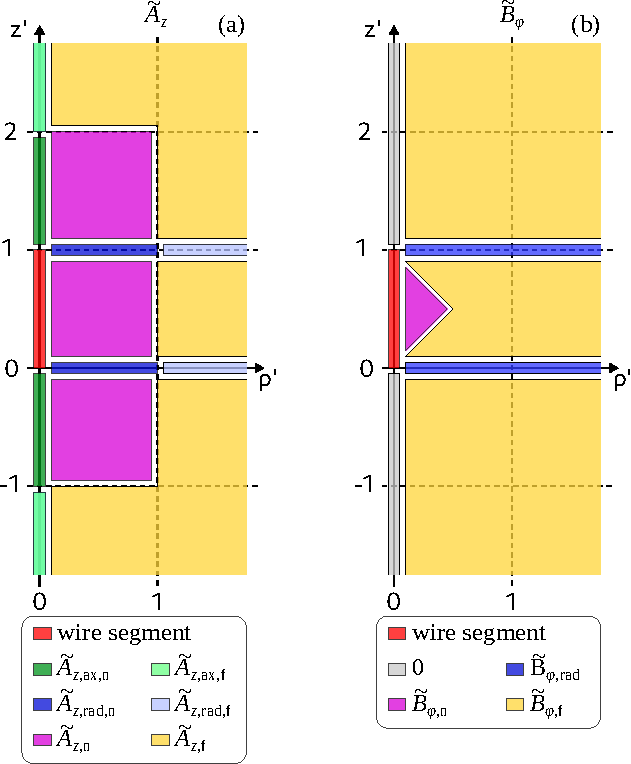
\includegraphics{img/sws_regions.pdf}
%     \includegraphics{img/figure_3.pdf}
    \caption{Domain decomposition used to partition the evaluation region
             for computing $\tilde{A}_z$ (a) and $\tilde{B}_\varphi$ (b) accurately.
             The colored regions indicate at which evaluation locations $(\rho',z')$
             which formulation (see legend) is used.}
    \label{fig:sws_regions}
\end{figure}

\FloatBarrier
\subsection{Circular Wire Loop}
\label{sec:methods_cwl}
The basic geometry of a circular wire loop under consideration here is shown in Fig.~\ref{fig:circularWireLoop}.
The loop is centered at the origin with its normal vector aligned with the $z$-axis.
The radius of the loop is denoted $a$ and a current $I$ (with corresponding current density~$\mathbf{j}$)
flows in the direction indicated in Fig.~\ref{fig:circularWireLoop}.
The magnetic field and vector potential are to be evaluated at the point $\mathbf{x}$ in the ($x$, $z$)-plane.
The coordinates of the evaluation point can be expressed in spherical coordinates as~$(r, \theta)$
or in cylindrical coordinates as~$(\rho, z)$.
The axisymmetry of this setup always allows to rotate the coordinate system such that $\varphi=0$ can be assumed.
\begin{figure}[htbp]
 \centering
 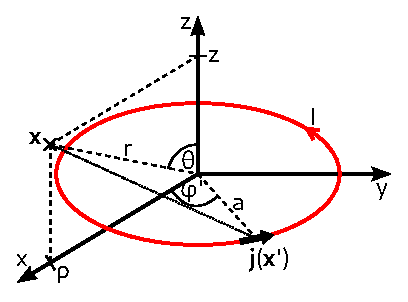
\includegraphics[width=0.5\textwidth]{img/circularWireLoop.eps}
%  \includegraphics[width=0.5\textwidth]{img/figure_4.eps}
 \caption{Geometry of a circular wire loop centered at the origin with normal vector aligned with the $z$-axis.}
 \label{fig:circularWireLoop}
\end{figure}
Similar to the case of the straight wire segment,
the magnetic vector potential and the magnetic field of the circular wire loop
are assembled from various formulations for special cases of the far-field and the near-field
in the implementation described later.

\subsubsection{Magnetic Vector Potential}
The magnetic vector potential of a circular wire loop
only has a tangential component~$A_\varphi$.
In Eqn.~(5.37) of Ref.~\cite{jackson}, $A_\varphi$~is expressed as
follows for a loop of radius~$a$ and current~$I$ along it:
\begin{align}
  A_\varphi(r, \theta) &= \frac{\mu_0}{4 \pi}
                          \frac{4 I a}{\sqrt{a^2 + r^2 + 2 a r \sin(\theta)}}
                          \left[
                            \frac{(2 - k^2)\mathcal{K}(k) - 2 \mathcal{E}(k)}{k^2}
                          \right] \label{eqn:cwl_A_phi_Jackson}
\end{align}
with
\begin{equation}
  k^2 = \frac{4 a r \sin(\theta)}{a^2 + r^2 + 2 a r \sin(\theta)} \, .
\end{equation}
Here, $\mathcal{K}(k)$ and $\mathcal{E}(k)$ are the complete elliptic integrals of the first and second kind, respectively.
Spherical coordinates~$(r, \theta)$ are used to specify the evaluation location.
The corresponding cylindrical coordinates~$(\rho, z)$ are given by
$\rho = r \sin(\theta)$ and $z = \sqrt{r^2 - \rho^2}$.
Normalized coordinates~$(\rho', z')$ are introduced with
\begin{align}
  \rho' =&\, \rho / a \label{eqn:rhoP} \\
    z'  =&\,   z  / a \label{eqn:zP}   \, .
\end{align}
An expression for the linear combination of $\mathcal{K}(k)$ and $\mathcal{E}(k)$
is used to reformulate \eqn{cwl_A_phi_Jackson}:
\begin{equation}
  \lambda \mathcal{K}(k) + \mu \mathcal{E}(k) = \,\mathrm{cel}(k_c, 1, \lambda + \mu, \lambda + \mu k_c^2) \label{eqn:K_E_by_cel}
\end{equation}
where
\begin{equation}
  k_\mathrm{c}^2 = 1 - k^2
\end{equation}
and cel is the so-called general complete elliptic integral
introduced by Bulirsch~\cite{bulirsch_3}:
\begin{equation}
  \mathrm{cel}(k_c, p, a, b) =
  \int\limits_0^{\pi/2}
    \frac{a \cos^2(\varphi) + b \sin^2(\varphi)}
         {\cos^2(\varphi) + p \sin^2(\varphi)}
    \frac{\mathrm{d}\varphi}
         {\sqrt{\cos^2(\varphi) + k_c^2 \sin^2(\varphi)}} \, .
\end{equation}
The argument of the elliptic integrals is considered first:
\begin{align}
  k^2 &= \frac{4 a r \sin(\theta)}{a^2 + r^2 + 2 a r \sin(\theta)}
       = \frac{4 a \rho}{a^2 + r^2 + 2 a \rho}
       = \frac{4 \bcancel{a} \rho}{a^{\bcancel{2}} \left(1 + \frac{r^2}{a^2} + 2 \frac{\rho}{a} \right)} \nonumber \\
  ~   &= \frac{4 \rho'}{1 + \frac{r^2}{a^2} + 2 \rho'}
       = 4 \rho' \left( 1 + \frac{\rho^2 + z^2}{a^2} + 2 \rho' \right)^{-1} \nonumber \\
  ~   &= 4 \rho' \left( 1 + \rho'^{2} + z'^{2} + 2 \rho' \right)^{-1}
       = \frac{4 \rho'}{z'^2 + (1 + \rho')^2} \, . \label{eqn:kSq}
\end{align}
This implies:
\begin{equation}
  k_c^2 = \frac{z'^2 + (1 - \rho')^2}{z'^2 + (1 + \rho')^2} \, . \label{eqn:kCSq_general}
\end{equation}
The coefficients of the elliptic integrals in \eqn{cwl_A_phi_Jackson} are identified as follows:
\begin{align}
  \lambda &= \frac{2 - k^2}{k^2} = \frac{2}{k^2} - 1 \\
  \mu     &= -\frac{2}{k^2}
\end{align}
and their combinations are as follows for use in \eqn{K_E_by_cel}:
\begin{align}
  \lambda + \mu       &= \frac{2}{k^2} - 1 - \frac{2}{k^2}     = -1 \\
  \lambda + \mu k_c^2 &= \frac{2}{k^2} - 1 - \frac{2}{k^2} (1 - k^2) \nonumber \\
          ~           &= \frac{2}{k^2} - 1 - \frac{2}{k^2} + 2 =  1 \label{eqn:lmkcsq} \, .
\end{align}
Putting Eqn.s~(\ref{eqn:K_E_by_cel}) to~(\ref{eqn:lmkcsq}) together, we arrive at the following expression for $A_\varphi$:
\begin{equation}
 A_\varphi(\rho', z') = \frac{\mu_0 I}{\pi}
                        \frac{1}{\sqrt{z'^2 + (1 + \rho')^2}} \,\mathrm{cel}(k_c, 1, -1, 1) \, . \label{eqn:cwl_A_phi_cel}
\end{equation}
It is favorable for numerical evaluation of $A_\varphi$ to use the form given in \eqn{cwl_A_phi_cel}
where the linear combination of the complete elliptic integrals is embedded in the parameters of cel
and less precautions need to be taken to deal with cancellations in \eqn{cwl_A_phi_Jackson}.
A physics-oriented prefactor is split off to be able to focus on geometry in the following:
\begin{equation}
  A_\varphi(\rho', z') = \frac{\mu_0 I}{\pi} \tilde{A}_\varphi(\rho',z') \label{eqn:norm_A_phi}
\end{equation}
with
\begin{equation}
  \tilde{A}_\varphi(\rho',z')
  = \frac{1}{\sqrt{z'^2 + (1 + \rho')^2}} \,\mathrm{cel}(k_c, 1, -1, 1) \, .
\end{equation}
One of several formulations for $\tilde{A}_\varphi$ is chosen depending on the evaluation location~$(\rho', z')$:
\begin{equation}
  \tilde{A}_\varphi (\rho', z') =
  \begin{cases}
    \textrm{undefined}                         &:\, \rho' = 1; z' = 0 \\
    0                                          &:\, \rho' = 0; \textrm{ any } z' \\
    \tilde{A}_{\varphi,\mathrm{f}} (\rho', z') &:\, (0 < \rho' < 1/2; \textrm{ any } z') \textrm{ or } \\
                   ~                           &~~     (\rho' > 2;   \textrm{ any } z') \textrm{ or } (\rho' > 0; |z'| \geq 1) \\
    \tilde{A}_{\varphi,\mathrm{v}} (z')        &:\, \rho' = 1; ( -1 < z' < 0 \textrm{ or } 0 < z' < 1) \\
    \tilde{A}_{\varphi,\mathrm{n}} (\rho', z') &:\, \textrm{elsewhere.}
  \end{cases} \label{eqn:A_phi_final}
\end{equation}
The domain decomposition used to compute $\tilde{A}_\varphi$ accurately is depicted in Fig.~\ref{fig:cwl_A_phi_regions}.
\begin{figure}[htbp]
    \centering
    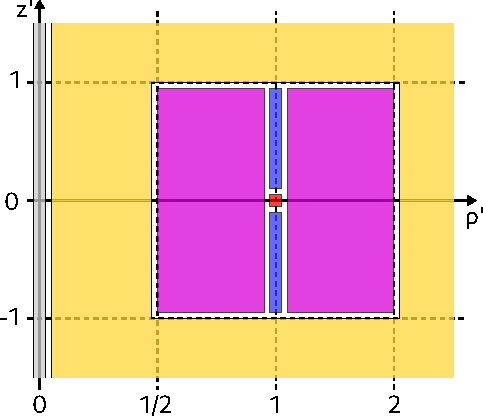
\includegraphics{img/cwl_A_phi_regions.pdf}
%     \includegraphics{img/figure_5.pdf}
    \caption{Domain decomposition used to partition the evaluation region
             for computing $\tilde{A}_\varphi$ accurately.
             The colored regions indicate at which evaluation locations $(\rho',z')$
             which formulation (see legend) is used.}
    \label{fig:cwl_A_phi_regions}
\end{figure}
The following formula is implemented for evaluation locations away from the wire loop:
\begin{equation}
  \tilde{A}_{\varphi,\mathrm{f}} (\rho',z')
  = \frac{k^2}{\sqrt{z'^2 + (1 + \rho')^2}} \,\mathcal{C}(k_c) \label{eqn:cwl_A_phi_f}
\end{equation}
with $k^2$~from~\eqn{kSq} and
\begin{equation}
  \mathcal{C}(k_c)
  = \,\mathrm{cel} \left( \frac{2 \sqrt{k_c}}{1 + k_c}, 1, 0, \frac{2}{(1 + k_c)^3} \right) \, . \label{eqn:elliptic_c}
\end{equation}
The derivation for this formulation is found in \eqn{cwl_A_phi_f_derivation}.
Close to the wire loop, the following formulation is used:
\begin{equation}
  \tilde{A}_{\varphi,\mathrm{n}} (\rho',z')
  = \frac{1}{|\rho' - 1| \sqrt{\left( \frac{z'}{\rho'-1} \right)^2 + \left(1 + \frac{2}{\rho'-1} \right)^2 }}
    \,\mathrm{cel}(\sqrt{k_c^2}, 1, -1, 1) \label{eqn:cwl_A_phi_n}
\end{equation}
with $k_c^2$ computed as follows:
\begin{equation}
  k_c^2 = \frac{\left( \frac{z'}{\rho'-1} \right)^2 + 1}{\left( \frac{z'}{\rho'-1} \right)^2 + \left(1 + \frac{2}{\rho'-1} \right)^2} \, .
\end{equation}
The derivation for this formulation is found in \eqn{cwl_A_phi_near}.
At~$\rho' = 1$, some further simplification can be carried out.
This leads to the following formulation for~$\rho' = 1$ and~$|z'| < 1$:
\begin{equation}
  \tilde{A}_{\varphi,\mathrm{v}} (z') = \frac{1}{|z'|} \,\mathrm{cel}\left(\frac{1}{k_c}, 1, 1, -1\right) \label{eqn:cwl_A_phi_v}
\end{equation}
with $k_c$ computed as follows:
\begin{equation}
  k_c = \frac{|z'|}{\sqrt{4 + {z'}^2}} \, ,
\end{equation}
which is derived in \eqn{cwl_A_phi_v_derivation}.

\subsubsection{Magnetic Field}
The magnetic field produced by a circular wire loop is made up of two components:
\begin{equation}
  \mathbf{B} = B_\rho \hat{\mathbf{e}}_\rho + B_z \hat{\mathbf{e}}_z
\end{equation}
where $B_\rho$ denotes the radial component and $B_z$ denotes the vertical component.
The radial component~$B_\rho$ is given by~\cite{teal}:
\begin{equation}
  B_\rho(\rho', z')
  = \frac{\mu_0 I}{\pi a} \frac{z'}{\left[ z'^2 + (1 + \rho')^2 \right]^{3/2}} \,\mathrm{cel}(k_c, k_c^2, -1, 1)
\end{equation}
Also here, a normalization factor is split off:
\begin{equation}
  B_\rho(\rho', z') = \frac{\mu_0 I}{\pi a} \tilde{B}_\rho(\rho', z')
\end{equation}
with
\begin{align}
  \tilde{B}_\rho(\rho', z')
  =&\, \frac{z'}{\left[ z'^2 + (1 + \rho')^2 \right]^{3/2}} \,\mathrm{cel}(k_c, k_c^2, -1, 1) \, .
\end{align}
One of several formulations is chosen depending on the evaluation location~$(\rho', z')$:
\begin{equation}
  \tilde{B}_\rho(\rho', z')
  = \begin{cases}
      \textrm{undefined}                      &:\, \rho' = 1; z' = 0 \\
      0                                       &:\, (\rho' = 0; \textrm{ any } z') \textrm{ or } (\rho' \neq 1; z' = 0) \\
      \tilde{B}_{\rho,\mathrm{f}} (\rho', z') &:\, \rho' > 0 \textrm{ and } |z'| > 0 \textrm{ and } \\
                     ~                        &~~ (\rho' < 1/2 \textrm{ or } \rho' > 2 \textrm{ or } |z'| \geq 1 ) \\
      \tilde{B}_{\rho,\mathrm{v}} (z')        &:\, \rho' = 1; ( -1 < z' < 0 \textrm{ or } 0 < z' < 1) \\
      \tilde{B}_{\rho,\mathrm{n}} (\rho', z') &:\, \textrm{elsewhere.}
    \end{cases} \label{eqn:cwl_B_rho_switchover}
\end{equation}
The domain decomposition used to compute $\tilde{B}_\rho$ accurately is depicted in Fig.~\ref{fig:cwl_B_rho_regions}.
\begin{figure}[htbp]
    \centering
    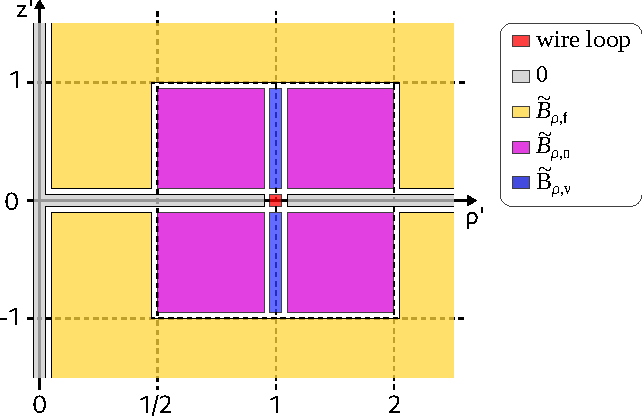
\includegraphics{img/cwl_B_rho_regions.pdf}
%     \includegraphics{img/figure_6.pdf}
    \caption{Domain decomposition used to partition the evaluation region
             for computing $\tilde{B}_\rho$ accurately.
             The colored regions indicate at which evaluation locations $(\rho',z')$
             which formulation (see legend) is used.}
    \label{fig:cwl_B_rho_regions}
\end{figure}
The following formulation is implemented for evaluation locations away from to the wire loop:
\begin{equation}
  \tilde{B}_{\rho,\mathrm{f}} (\rho', z')
  = \frac{4 \rho' z' \left[ \,\mathcal{D}(k_c) - \,\mathcal{C}(k_c) \right]}
         {\left[{z'}^2 + (1 + \rho')^2 \right]^{3/2} \left[{z'}^2 + (1 - \rho')^2 \right] } \label{eqn:cwl_B_rho_f}
\end{equation}
with
\begin{equation}
  \mathcal{D}(k_c)
  = \frac{\mathcal{K}(k) - \,\mathcal{E}(k)}{k^2}
  = \,\mathrm{cel}(k_c, 1, 0, 1) \, . \label{eqn:elliptic_d}
\end{equation}
The derivation for this formulation is found in \eqn{cwl_B_rho_f_derivation}.
For points close to the wire loop, but with~$\rho' \neq 1$, the following formulation is used:
\begin{align}
  \tilde{B}_{\rho,\mathrm{n}}& (\rho', z')
  = \frac{4 \rho' \frac{z'}{|\rho'-1|} \left[ \,\mathcal{D}(k_c) - \,\mathcal{C}(k_c) \right]}
         {(\rho' - 1)^4} \nonumber \\
  ~& \left\{
      \left[ \left( \frac{z'}{\rho'-1} \right)^2 + \left(1 + \frac{2}{\rho'-1} \right)^2 \right]^{3/2}
      \left[ \left( \frac{z'}{\rho'-1} \right)^2 + 1 \right]
    \right\}^{-1} \label{eqn:cwl_B_rho_n} \, .
\end{align}
The derivation for this formulation is found in \eqn{cwl_B_rho_n_derivation}.
Finally, for $\rho'=1$ and~$|z'| < 1$, the following formulation is used:
\begin{equation}
  \tilde{B}_{\rho,\mathrm{v}} (z')
  = \frac{k_c}{2} \frac{z'}{|z'|} \left[ \left( \frac{2}{z'^2} + 1 \right) \mathcal{E}(k_c) - \mathcal{K}(k_c) \right] \label{eqn:cwl_B_rho_v}
\end{equation}
with
\begin{equation}
  k_c^2 = \frac{1}{1 + 4/{z'}^2}
\end{equation}
and
\begin{align}
  \mathcal{K}(k_c) =&\, \,\mathrm{cel}(k_c, 1, 1, 1) \\
  \mathcal{E}(k_c) =&\, \,\mathrm{cel}(k_c, 1, 1, k_c^2) \, .
\end{align}
The derivation for this formulation is found in \eqn{cwl_B_rho_v_derivation}.
The vertical component~$B_z$ of the magnetic field of a circular wire loop is given by~\cite{teal}:
\begin{align}
 B_z(\rho', z')
 =&\, \frac{\mu_0 I}{2 \pi a}
   \frac{1}{\rho' \sqrt{z'^2 + (1 + \rho')^2}} \nonumber \\
 ~& \left[
       \textrm{cel}(k_c, 1, -1, 1)
     + \frac{1 + k_c^2 - \left( 1 - k_c^2 \right) \rho'}{2} \textrm{cel}(k_c, k_c^2, -1, 1)
   \right]
\end{align}
A normalization factor is split off here as well:
\begin{equation}
  B_z(\rho', z') = \frac{\mu_0 I}{\pi a} \tilde{B}_z(\rho', z')
\end{equation}
with
\begin{align}
  \tilde{B}_z(\rho', z')
  =&\, \frac{1}{2 \rho' \sqrt{z'^2 + (1 + \rho')^2}} \nonumber \\
 ~& \left[
       \textrm{cel}(k_c, 1, -1, 1)
     + \frac{1 + k_c^2 - \left( 1 - k_c^2 \right) \rho'}{2} \textrm{cel}(k_c, k_c^2, -1, 1)
   \right] \, .
\end{align}
The evaluation of this formula is split up as well into separate special cases.
One of several formulations is selected depending on the evaluation location~$(\rho', z')$:
\begin{equation}
  \tilde{B}_z(\rho', z')
  = \begin{cases}
      \textrm{undefined}                    &:\, \rho' = 1; z' = 0 \\
      \tilde{B}_{z,\mathrm{f1}} (\rho', z') &:\, (\rho' < 1/2; \textrm{ any } z') \textrm{ or } \\
                ~                           &~~  (\rho' \leq 2; |z'| > 1) \\
      \tilde{B}_{z,\mathrm{f2}} (\rho', z') &:\, \rho' > 2, \textrm{ any } z' \\
      \tilde{B}_{z,\mathrm{v}}  (z')        &:\, \rho' = 1; ( -1 \leq z' < 0 \textrm{ or } 0 < z' \leq 1) \\
      \tilde{B}_{z,\mathrm{n}}  (\rho', z') &:\, \textrm{elsewhere.} \\
    \end{cases} \label{eqn:cwl_B_z_switchover}
\end{equation}
The domain decomposition used to compute $\tilde{B}_z$ accurately is depicted in Fig.~\ref{fig:cwl_B_z_regions}.
\begin{figure}[htbp]
    \centering
    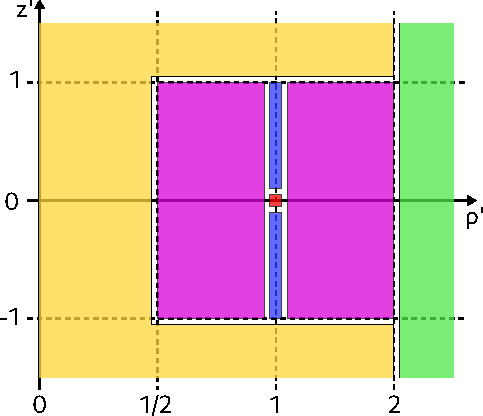
\includegraphics{img/cwl_B_z_regions.pdf}
%     \includegraphics{img/figure_7.pdf}
    \caption{Domain decomposition used to partition the evaluation region
             for computing $\tilde{B}_z$ accurately.
             The colored regions indicate at which evaluation locations $(\rho',z')$
             which formulation (see legend) is used.}
    \label{fig:cwl_B_z_regions}
\end{figure}
For points not too close to the wire loop and with $\rho' \leq 2$, the following formulation is used:
\begin{align}
  \tilde{B}_{z,\mathrm{f1}} (\rho', z')
  =&\, \frac{1}{\sqrt{{z'}^2 + (1+\rho')^2} \left[{z'}^2 + (1 - \rho')^2 \right] } \nonumber \\
  ~&\,  \left\{ \mathcal{E}(k_c) + \rho' \left[ \mathcal{E}(k_c) - 2 \mathcal{K}(k_c) + 2 \mathcal{D}(k_c) \right] \right\} \, . \label{eqn:cwl_B_z_f1}
\end{align}
The derivation for this formulation is found in \eqn{cwl_B_z_f1_appendix}.
A second far-field method is needed for points with $\rho' > 2$:
\begin{equation}
  \tilde{B}_{z,\mathrm{f2}} (\rho', z')
  = \frac{1}{\sqrt{t_1 + t_2}(t_1-t_2) {\rho'}^3}
    \left\{ \mathcal{E}(k_c) + \frac{4}{\alpha_\mathrm{cd}} \left[ \mathcal{C}(k_c) - \,\mathcal{D}(k_c) \right] \right\} \label{eqn:cwl_B_z_f2}
\end{equation}
with
\begin{align}
  t_1 =&\, \frac{z'^2 + 1}{\rho'^2} + 1 \\
  t_2 =&\, \frac{2}{\rho'}
\end{align}
and
\begin{equation}
  \alpha_\mathrm{cd} = 1 + \frac{1}{\rho'} \left[ 2 + \frac{1}{\rho'} \left( 1 + {z'}^2 \right) \right] \, .
\end{equation}
The derivation for this formulation is found in \eqn{cwl_B_z_f2_derivation}.
In the vicinity of the wire loop, but with $z' \neq 0$,
the following method is used to compute $\tilde{B}_z$:
\begin{equation}
  \tilde{B}_{z,\mathrm{n}} (\rho', z')
  = \frac{\,\mathrm{cel}\left( \sqrt{k_c^2}, k_c^2, 1 + \rho', 1 - \rho' \right) }
         {\left|\rho' - 1 \right|^3 \left[ \left( \frac{z'}{\rho'-1} \right)^2 + \left(1 + \frac{2}{\rho'-1} \right)^2 \right]^{3/2} } \, . \label{eqn:cwl_B_z_n}
\end{equation}
The derivation for this formulation is found in \eqn{cwl_B_z_n_derivation}.
The expression for $\tilde{B}_z$ becomes significantly simpler at $\rho'=1$,
which is considered next:
\begin{equation}
  \tilde{B}_{z,\mathrm{v}} (z')
  = \frac{1}{\left[ {z'}^2 + 4 \right]^{3/2}} \,\mathrm{cel}\left(\sqrt{k_c^2}, k_c^2, 2, 0 \right) \label{eqn:cwl_B_z_v}
\end{equation}
with
\begin{equation}
  k_c^2 = \frac{{z'}^2}{{z'}^2 + 4} \, .
\end{equation}
The derivation for this formulation is found in \eqn{cwl_B_z_v_derivation}.

\FloatBarrier
\subsection{Evaluation in Global Coordinates}
Evaluation of the magnetic vector potential~$\mathbf{A}$ and magnetic field~$\mathbf{B}$
produced by the current carriers considered in this work
happens in cylindrical coordinates~$\rho$ and~$z$
in the local coordinate system of the current carriers.
It is often more convenient to be able to work in global coordinates.
The methods given in this section show how to transform the evaluation location
into cylindrical coordinates in the frame of reference of the current carrier
and subsequently transform back the magnetostatic quantities into the global global coordinate system.

\subsubsection{Straight Wire Segment}
Figure~\ref{fig:StraightWireSegment_MappingToCartesian} illustrates the setup for a straight wire segment.
\begin{figure}[htbp]
 \centering
 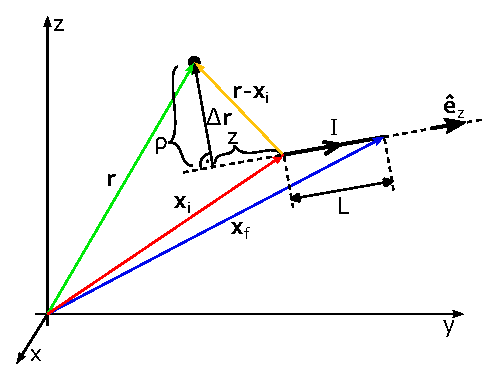
\includegraphics{img/StraightWireSegment_MappingToCartesian.eps}
%  \includegraphics{img/figure_8.eps}
 \caption{Mapping the components to global coordinates for an exemplary straight wire segment.
          The wire segment is positioned from~$\mathbf{x}_\mathrm{i}$ to~$\mathbf{x}_\mathrm{f}$.
          Its parallel unit vector is denoted $\hat{\mathbf{e}}_z$.
          The length of the wire segment is denoted by~$L$.
          The evaluation location is denoted by~$\mathbf{r}$.}
 \label{fig:StraightWireSegment_MappingToCartesian}
\end{figure}
The length of the wire segment is denoted by~$L$:
\begin{equation}
  L = |\mathbf{x}_f - \mathbf{x}_i| \, .
\end{equation}
If $L=0$, no contribution is taken into account from the wire segment.
Otherwise, the unit vector along the segment~$\hat{\mathbf{e}}_z$ is computed as:
\begin{equation}
  \hat{\mathbf{e}}_z = \frac{\mathbf{x}_f - \mathbf{x}_i}{L} \, .
\end{equation}
The vertical coordinate~$z$ in the coordinate system of the wire segment is:
\begin{equation}
  z = (\mathbf{r} - \mathbf{x}_i) \cdot \hat{\mathbf{e}}_z
\end{equation}
and the normalized $z$-coordinate is:
\begin{equation}
  z' = \frac{z}{L} = \frac{1}{L} (\mathbf{r} - \mathbf{x}_i) \cdot \hat{\mathbf{e}}_z \, .
\end{equation}
For the radial coordinate, first the vector~$\Delta \mathbf{r}$ is formed:
\begin{equation}
  \Delta \mathbf{r} = (\mathbf{r} - \mathbf{x}_i) - z \, \hat{\mathbf{e}}_z
\end{equation}
and the radial coordinate $\rho$ is then obtained by taking $\rho = |\Delta \mathbf{r}|$.
The normalized radial coordinate~$\rho'$ is then obtained as:
\begin{equation}
  \rho' = \frac{\rho}{a} = \frac{1}{a} |(\mathbf{r} - \mathbf{x}_i) - z \, \hat{\mathbf{e}}_z| \, .
\end{equation}
The magnetic vector potential only has a component in parallel direction in the coordinate system of the wire segment.
The vector potential of the circular wire loop in thus in Cartesian coordinates:
\begin{equation}
  \mathbf{A}(\mathbf{r}) = A_z(\rho', z') \hat{\mathbf{e}}_z \, .
\end{equation}
If $\rho' \neq 0$, a unit vector in radial direction is formed as follows:
\begin{equation}
  \hat{\mathbf{e}}_\rho = \frac{\Delta \mathbf{r}}{\rho}
\end{equation}
and the magnetic field of the straight wire segment (consisting only of the tangential component~$B_\varphi$)
is evaluated as:
\begin{equation}
  \mathbf{B}(\mathbf{r}) = B_\varphi(\rho', z') \hat{\mathbf{e}}_\varphi
\end{equation}
with $\hat{\mathbf{e}}_\varphi = \hat{\mathbf{e}}_z \times \hat{\mathbf{e}}_\rho$.

\subsubsection{Circular Wire Loop}
Figure~\ref{fig:CircularWireLoop_MappingToCartesian} illustrates the setup of a circular wire loop.
\begin{figure}[htbp]
 \centering
 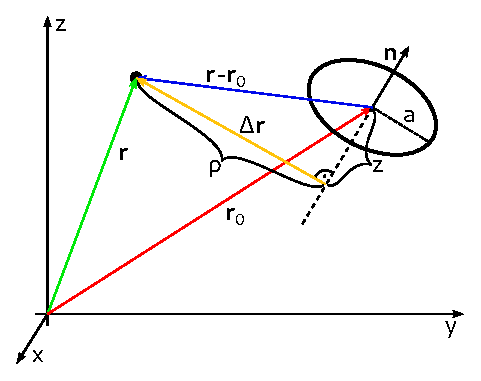
\includegraphics{img/CircularWireLoop_MappingToCartesian.eps}
%  \includegraphics{img/figure_9.eps}
 \caption{Mapping the components to Cartesian coordinates for an exemplary circular wire loop.
          The loop is centered around its origin~$\mathbf{r}_0$.
          Its normal vector is denoted $\mathbf{n}$ and defines the orientation of the loop.
          The radius of the loop is denoted by~$a$.
          The evaluation location is denoted by~$\mathbf{r}$.}
 \label{fig:CircularWireLoop_MappingToCartesian}
\end{figure}
The $z$-axis of the coordinate system of the wire loop is defined by the normal vector~$\mathbf{n}$:
\begin{equation}
  \hat{\mathbf{e}}_z = \frac{\mathbf{n}}{|\mathbf{n}|} \, .
\end{equation}
The $z$ component of the evaluation location is thus obtained as follows:
\begin{equation}
  z = (\mathbf{r} - \mathbf{r}_0) \cdot \hat{\mathbf{e}}_z \, .
\end{equation}
The normalized $z$-coordinate $z'$ is then obtained as:
\begin{equation}
  z' = \frac{z}{a} = \frac{1}{a} (\mathbf{r} - \mathbf{r}_0) \cdot \hat{\mathbf{e}}_z \, .
\end{equation}
For the radial coordinate, first the vector~$\Delta \mathbf{r}$ is formed:
\begin{equation}
  \Delta \mathbf{r} = (\mathbf{r} - \mathbf{r}_0) - z \, \hat{\mathbf{e}}_z
\end{equation}
and the radial coordinate $\rho$ is then obtained by taking $\rho = |\Delta \mathbf{r}|$.
The normalized radial coordinate~$\rho'$ is then obtained as:
\begin{equation}
  \rho' = \frac{\rho}{a} = \frac{1}{a} |(\mathbf{r} - \mathbf{r}_0) - z \, \hat{\mathbf{e}}_z| \, .
\end{equation}
The magnetic field of the circular wire loop consists of two cylindrical components, namely $B_\rho$ and $B_z$.
The Cartesian magnetic field components are then computed as follows:
\begin{equation}
  \mathbf{B}(\mathbf{r}) = B_\rho(\rho', z') \hat{\mathbf{e}}_\rho + B_z(\rho', z') \hat{\mathbf{e}}_z \, .
\end{equation}
If $\rho' = 0$, only $B_z$ is evaluated.
Otherwise, a unit vector in radial direction is formed as follows:
\begin{equation}
  \hat{\mathbf{e}}_\rho = \frac{\Delta \mathbf{r}}{\rho}
\end{equation}
and $B_\rho$ is evaluated as well.
The magnetic vector potential only has a component in tangential direction in the coordinate system of the wire loop.
It is also only evaluated if $\rho' \neq 0$.
The corresponding unit vector~$\hat{\mathbf{e}}_\varphi$ is then given by
$\hat{\mathbf{e}}_\varphi = \hat{\mathbf{e}}_z \times \hat{\mathbf{e}}_\rho$.
The vector potential of the circular wire loop in thus in Cartesian coordinates:
\begin{equation}
  \mathbf{A}(\mathbf{r}) = A_\varphi(\rho', z') \hat{\mathbf{e}}_\varphi \, .
\end{equation}

\FloatBarrier
\subsection{Verification Method}
\label{sec:methods_verification}
The implementations of above formulas for the magnetic vector potential
and magnetic field of a straight wire segment and a circular wire loop
need to be tested before using the implementations in routine work.
This section introduces the choice of test point coordinates.
A rectangular grid of test points in the $(\rho', z')$-plane is defined,
where the choice of knots along the $\rho'$ and $z'$ axes are discussed below.
The set of test point coordinates for testing a given current carrier primitive
consists of the combinations of all test knots along the $\rho'$ axis
with all test knots along the $z'$ axis.
Let $T_{\rho'}$ ($T_{z'}$) be the set of knots along the $\rho'$ ($z'$) axis to test the formulation on.
Then $T = T_{\rho'} \otimes T_{z'} \\ T_\mathrm{cc}$ is the set of test point coordinates
where $\otimes$ is the cartesian product of two sets
and $T_\mathrm{cc}$ is the subset of points from $T_{\rho'} \otimes T_{z'}$ that are located exactly on the current carrier.
First, the choice of test points for testing the implementations
of the straight wire segment methods~(SWS) is introduced.
The set of grid knots along the $\rho'$ axis, $T^\mathrm{SWS}_{\rho'}$, are chosen as follows:
\begin{itemize}
  \item $T^\mathrm{SWS}_{\rho',1} = \{ 0 \}$
  \item $T^\mathrm{SWS}_{\rho',2} = \{ 10^{-30}, 10^{-29}, ..., 10^{30} \}$
\end{itemize}
with $T^\mathrm{SWS}_{\rho'} = T^\mathrm{SWS}_{\rho',1} \cup T^\mathrm{SWS}_{\rho',2}$,
leading to $|T^\mathrm{SWS}_{\rho'}| = 62$.
The set of grid knots along the $z'$ axis, $T^\mathrm{SWS}_{z'}$, are chosen as follows:
\begin{itemize}
  \item $T^\mathrm{SWS}_{z',1} = \{ -10^{30}, -10^{29}, ..., -10^{-30} \}$
  \item $T^\mathrm{SWS}_{z',2} = \{ 10^{-30}, 10^{-29}, ..., 10^{-1} \}$
  \item $T^\mathrm{SWS}_{z',3} = \{ 1 - 10^{-1}, 1 - 10^{-2}, ..., 1 - 10^{-15}, 1 - \epsilon_{64}/2 \}$
  \item $T^\mathrm{SWS}_{z',4} = \{ 1 + \epsilon_{64}, 1 + 10^{-15}, 1 + 10^{-14}, ..., 1 + 10^{-1} \}$
  \item $T^\mathrm{SWS}_{z',5} = \{ 10^{1}, 10^{2}, ..., 10^{30} \}$
  \item $T^\mathrm{SWS}_{z',6} = \{ 0, 1/2, 1, 2 \}$
\end{itemize}
with $T^\mathrm{SWS}_{z'} = T^\mathrm{SWS}_{z',1} \cup T^\mathrm{SWS}_{z',2} \cup T^\mathrm{SWS}_{z',3} \cup T^\mathrm{SWS}_{z',4} \cup T^\mathrm{SWS}_{z',5} \cup T^\mathrm{SWS}_{z',6}$,
leading to $|T^\mathrm{SWS}_{z'}| = 157$.
The machine-precision epsilon is given by $\epsilon_{64} \approx 2.2 \times 10^{-16}$ for the case of \texttt{binary64}.
The exclusion of the test points that are located exactly on the wire segment leads to
a total number of test point coordinates~$T_\mathrm{SWS}$ for the straight wire segment of
$|T_\mathrm{SWS}| = 9685$.
Next, the choice of test points for testing the implementations
of the circular wire loop~(CWL) methods is introduced.
The set of grid knots along the $\rho'$ axis, $T^\mathrm{CWL}_{\rho'}$, are chosen as follows:
\begin{itemize}
  \item $T^\mathrm{CWL}_{\rho',1} = \{ 10^{-30}, 10^{-29}, ..., 10^{-1} \}$
  \item $T^\mathrm{CWL}_{\rho',2} = \{ 1 - 10^{-1}, 1 - 10^{-2}, ..., 1 - 10^{-15}, 1 - \epsilon_{64}/2 \}$
  \item $T^\mathrm{CWL}_{\rho',3} = \{ 1 + \epsilon_{64}, 1 + 10^{-15}, 1 + 10^{-14}, ..., 1 + 10^{-1} \}$
  \item $T^\mathrm{CWL}_{\rho',4} = \{ 10^{1}, 10^{2}, ..., 10^{30} \}$
  \item $T^\mathrm{CWL}_{\rho',5} = \{ 0, 1/2, 1, 2 \}$
\end{itemize}
with $T^\mathrm{CWL}_{\rho'} = T^\mathrm{CWL}_{\rho',1} \cup T^\mathrm{CWL}_{\rho',2} \cup T^\mathrm{CWL}_{\rho',3} \cup T^\mathrm{CWL}_{\rho',4} \cup T^\mathrm{CWL}_{\rho',5}$,
leading to $|T^\mathrm{CWL}_{\rho'}| = 96$.
The set of grid knots along the $z'$ axis, $T^\mathrm{CWL}_{z'}$, are chosen as follows:
\begin{itemize}
  \item $T^\mathrm{CWL}_{z',1} = \{ 0 \}$
  \item $T^\mathrm{CWL}_{z',2} = \{ 10^{-30}, 10^{-29}, ..., 10^{30} \}$
\end{itemize}
with $T^\mathrm{CWL}_{z'} = T^\mathrm{CWL}_{z',1} \cup T^\mathrm{CWL}_{z',2}$,
leading to $|T^\mathrm{CWL}_{z'}| = 62$.
The exclusion of the test point that is located exactly on the wire loop leads to
a total number of test point coordinates~$T_\mathrm{CWL}$ for the circular wire loop of
$|T_\mathrm{CWL}| = 5951$.
The reference results are computed on each test point using arbitrary-precision arithmetic
as provided by the Python package~\texttt{mpmath}~\cite{mpmath} and Mathematica~\cite{Mathematica}.
The test point coordinates are computed within the finite-precision test programs used to check the accuracy of the results.
This implies that the exact \textit{implied} values of the test point coordinates have to be transported
into the arbitrary-precision software used to compute the reference data.
The evaluation positions are specified at IEEE754~\texttt{binary64} floating-point numbers.
The floating point numbers are re-constructed within the arbitrary-precision software
in order to properly transport their intended value.
In case of \texttt{binary64}, this is done as follows for a floating-point number~$f$:
\begin{equation}
 f(s, E, M) =
 \begin{cases}
   0                                                             &: E=0 \textrm{ and } M=0 \\
   (-1)^s \, 2^{E - 1023} \, \left( 1 + \frac{M}{2^{52}} \right) &: \textrm{else}
  \end{cases} \label{eqn:binary64}
\end{equation}
where $s$ is the sign bit, $E$ is the exponent specified as an 11-bit unsigned integer
and $M$ is the mantissa specified as a 52-bit unsigned integer.
Several special cases are defined for certain values of $s$, $E$ and $M$,
but in the context of this work only the case $E=0$, $M=0$ ($s$ arbitrary),
which represents an exact zero, is relevant.
The organization of those bits in a \texttt{binary64} number is shown in Fig.~\ref{fig:binary64}.
\begin{figure}[htbp]
 \centering
 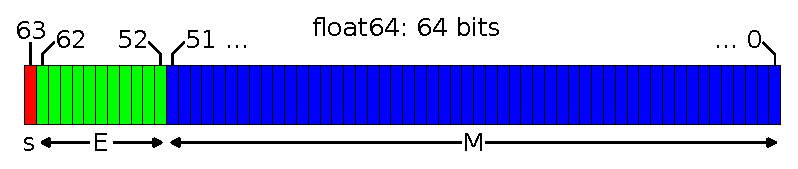
\includegraphics{img/IEEE754_binary64.eps}
%  \includegraphics{img/figure_10.eps}
 \caption{Organization of sign bit~$s$, exponent~$E$ (11 bits, unsigned integer)
          and mantissa~$M$ (52 bits, unsigned integer) within the 64 bits
          of a IEEE754~\texttt{binary64} floating-point number.
          Each box represents one bit and the colors indicate which quantity a bit belongs to
          (red: sign bit, green: exponent, blue: mantiassa).}
 \label{fig:binary64}
\end{figure}
In particular, a test point coordinate value~$f$ is passed to the reference computation
by passing the three values $s$, $E$ and $M$ as integers (which are easy to represent exactly).
Within the reference computation, the value of $f$ is constructed using~\eqn{binary64} implemented
in arbitrary precision and with the exact values of $s$, $E$ and $M$.
The reference data for the straight wire segment methods
is computed using 300 decimal digits of precision.
The reference data for the circular wire loop
is computed using 200 decimal digits of precision.
The evaluation position is specified exactly
via $s_\rho$, $E_\rho$ and $M_\rho$ (for $\rho'$)
and $s_z$, $E_z$ and $M_z$ (for $z'$):
\begin{align}
 \rho' \leftarrow&\, \begin{cases}
                       0  &:\, E_\rho = 0 \textrm{ and } M_\rho = 0 \\
                       (-1)^{s_\rho} \, 2^{E_\rho - 1023} \, \left(1 + M_\rho / 2^{52}  \right) &:\, \textrm{else}
                     \end{cases} \nonumber \\
    z' \leftarrow&\, \begin{cases}
                       0  &:\, E_z = 0 \textrm{ and } M_z = 0 \\
                       (-1)^{s_z   } \, 2^{E_z    - 1023} \, \left(1 + M_z / 2^{52}  \right) &:\, \textrm{else}
                     \end{cases} \nonumber
\end{align}
The following algorithm is used to compute reference values
of $\tilde{A}_z$ and $\tilde{B}_\varphi$ at~$(\rho', z')$
for the straight wire segment:
\begin{align}
  r_\mathrm{i}  \leftarrow&\, \sqrt{ {\rho'}^2 + {z'}^2 } \nonumber \\
  r_\mathrm{f}  \leftarrow&\, \sqrt{ {\rho'}^2 + \left(1 - z'\right)^2 } \nonumber \\
  \epsilon \leftarrow&\, \left( r_\mathrm{i} + r_\mathrm{f} \right)^{-1} \nonumber \\
  \tilde{A}_z \leftarrow&\, \textrm{atanh} (\epsilon) \label{eqn:sws_A_z_ref} \\
  \tilde{B}_\varphi \leftarrow&\, \left(\frac{1}{r_\mathrm{i}} + \frac{1}{r_\mathrm{f}} \right) \frac{\rho'}{r_\mathrm{i} r_\mathrm{f} + {\rho'}^2 + z' (z' - 1)} \label{eqn:sws_B_phi_ref}
\end{align}
The following algorithm is used to compute reference values
of $\tilde{A}_\varphi$ and $\tilde{B}_\rho$ at~$(\rho', z')$
for the circular wire loop:
\begin{align}
 k_c^2 \leftarrow&\, \frac{{z'}^2 + \left(1 - \rho'\right)^2}{{z'}^2 + \left(1 + \rho'\right)^2} \nonumber \\
 \tilde{A}_\varphi \leftarrow&\,
 \begin{cases}
   0 &:\, \rho' = 0 \\
   \frac{1}{\sqrt{{z'}^2 + \left(1 + \rho'\right)^2}}
                                 \int\limits_0^{\pi/2}
                                   \frac{\sin^2(\varphi) - \cos^2(\varphi)}
                                        {\sqrt{\cos^2(\varphi) + k_c^2 \sin^2(\varphi)}} \,\mathrm{d}\varphi &:\, \textrm{else}
 \end{cases} \label{eqn:A_phi_ref} \\
 \tilde{B}_\rho \leftarrow&\,
 \begin{cases}
   0 &:\, \rho' = 0 \textrm{ or } z' = 0 \\
   \frac{z'}{\left[{z'}^2 + \left(1 + \rho'\right)^2\right]^{3/2}}
                                 \int\limits_0^{\pi/2}
                                   \frac{\sin^2(\varphi) - \cos^2(\varphi)}
                                        {\left[\cos^2(\varphi) + k_c^2 \sin^2(\varphi)\right]^{3/2}} \,\mathrm{d}\varphi &:\, \textrm{else}
 \end{cases} \label{eqn:B_rho_ref}
\end{align}
The method used to compute $\tilde{B}_z$ works slightly differently:
\begin{align}
 k^2 \leftarrow&\,
  \begin{cases}
    4 / \left( \frac{1}{\rho'} + 2 + \rho' \right)    &: z' = 0 \\
    \frac{4 \rho'}{{z'}^2 + \left(1 + \rho'\right)^2} &: \textrm{else}
  \end{cases} \nonumber \\
 \tilde{B}_z \leftarrow&\,
   \frac{1}{\left[ {z'}^2 + \left(1 + \rho'\right)^2 \right]^{3/2} }
                                 \int\limits_0^{\pi/2}
                                   \frac{(1-\rho') \sin^2(\varphi) + (1+\rho') \cos^2(\varphi)}
                                        {\left[1 - k^2 \sin^2(\varphi) \right]^{3/2}} \,\mathrm{d}\varphi  \label{eqn:B_z_ref}
\end{align}
The integrals are carried out numerically within the arbitrary-precision software.
In case of~\texttt{mpmath}, double-exponential quadrature~\cite{double_exp_quad} is used~\cite{mpmath_quad}.
The particular choices for the number of digits of precision used throughout the arbitrary-precision computation
mentioned above have been adjusted to robustly yield enough equal digits
in the outputs from \texttt{mpmath} and Mathematica for benchmarking the \texttt{binary64} implementation of the methods presented in Sec.~\ref{sec:methods_sws} and~\ref{sec:methods_cwl}.
The error metric employed in this work is given as follows:
\begin{equation}
 \delta(a, b)
 = \begin{cases}
    \log_{10} \left(\min\left(1, \left| \frac{a - b}{b} \right|\right) \right) &: b \neq 0, a \neq b \\
    0                                                                          &: b=0, a \neq 0 \\
    -16                                                                        &: \textrm{else}
   \end{cases} \label{eqn:error_metric}
\end{equation}
where the constant~$-16$ is chosen for \texttt{binary64} as $\lfloor \log_{10}(\epsilon_{64}) \rfloor$.
Here, $a$ is the value to be tested and
$b$ is the reference value computed using arbitrary-precision arithmetic.

\section{Results}
\label{sec:results}
The results of the verification method introduced in Sec.~\ref{sec:methods_verification}
are presented next.
\subsection{Straight Wire Segment}
First, the results of the verification of the straight wire segment methods are presented.
The normalized vertical component of the magnetic vector potential, $\tilde{A}_z$,
and the normalized tangential component magnetic field, $\tilde{B}_\varphi$, of a straight wire segment
have been evaluated using \eqn{sws_A_z_switchover} and \eqn{sws_B_phi_switchover}, respectively,
on all test points in $T_\mathrm{SWS}$ (see Sec.~\ref{sec:methods_verification}).
Fig.~(\ref{fig:StraightWireSegment_A_z_Java}) shows the deviation
according to the error metric~\eqn{error_metric}
between the reference data computed for $\tilde{A}_z$ using \eqn{sws_A_z_ref}
and the results from the \texttt{float64} implementation of \eqn{sws_A_z_switchover}.
\begin{figure}[htbp]
 \centering
 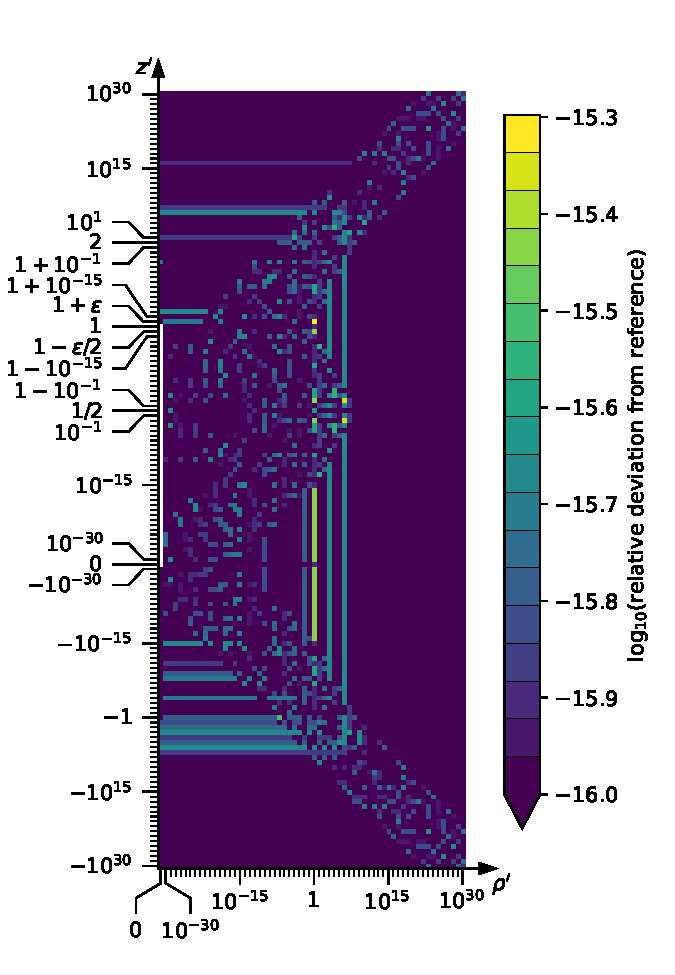
\includegraphics[height=0.8\textwidth]{img/StraightWireSegment_A_z_Java.pdf}
 \caption{Deviation between Java implementation of \eqn{sws_A_z_switchover} and \eqn{sws_A_z_ref}
          for the computation of $\tilde{A}_z$ of a straight wire segment
          in the error metric given by~\eqn{error_metric}.}
 \label{fig:StraightWireSegment_A_z_Java}
\end{figure}
It is observed that the relative error is less that $10^{-15}$ for all test points under consideration.
Fig.~(\ref{fig:StraightWireSegment_B_phi_Java}) shows the deviation
according to the error metric~\eqn{error_metric}
between the reference data computed for $\tilde{B}_\varphi$ using \eqn{sws_B_phi_ref}
and the results from the \texttt{float64} implementation of \eqn{sws_B_phi_switchover}.
\begin{figure}[htbp]
 \centering
 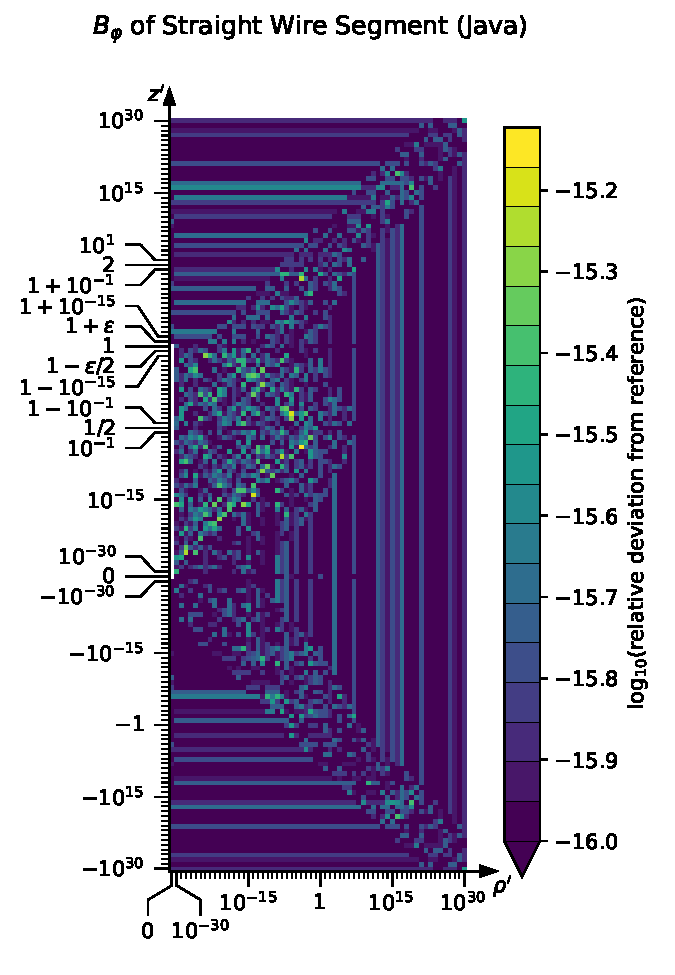
\includegraphics[height=0.8\textwidth]{img/StraightWireSegment_B_phi_Java.pdf}
 \caption{Deviation between Java implementation of \eqn{sws_B_phi_switchover} and \eqn{sws_B_phi_ref}
          for the computation of $\tilde{B}_\varphi$ of a straight wire segment
          in the error metric given by~\eqn{error_metric}.}
 \label{fig:StraightWireSegment_B_phi_Java}
\end{figure}
It is observed that the relative error is less that $10^{-15}$ for all test points under consideration.

\subsection{Circular Wire Loop}
Next, the results of the verification of the circular wire loop methods are presented.
The normalized tangential component of the magnetic vector potential, $\tilde{A}_\varphi$,
and the normalized radial and vertical components of the magnetic field, $\tilde{B}_\rho$ and $\tilde{B}_z$,
of a circular wire loop have been evaluated using \eqn{A_phi_final}, \eqn{cwl_B_rho_switchover}
and \eqn{cwl_B_z_switchover}, respectively,
on all test points in $T_\mathrm{CWL}$ (see Sec.~\ref{sec:methods_verification}).
Fig.~(\ref{fig:CircularWireLoop_A_phi_Java}) shows the deviation
according to the error metric~\eqn{error_metric}
between the reference data computed for $\tilde{A}_\varphi$ using \eqn{A_phi_ref}
and the results from the \texttt{float64} implementation of \eqn{A_phi_final}.
\begin{figure}[htbp]
 \centering
 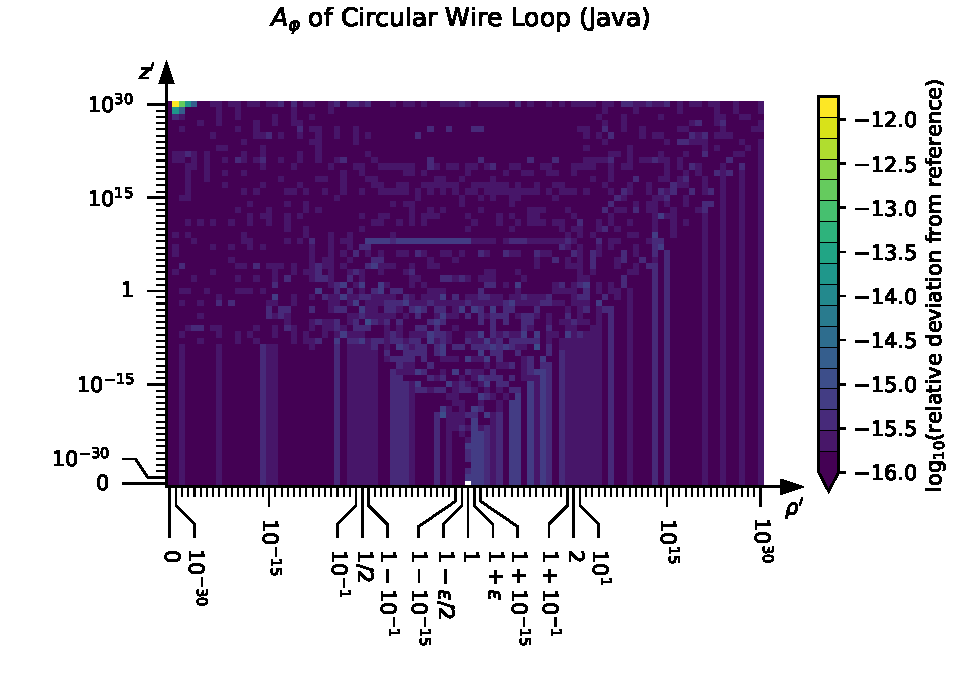
\includegraphics[width=0.8\textwidth]{img/CircularWireLoop_A_phi_Java.pdf}
 \caption{Deviation between Java implementation of \eqn{A_phi_final} and \eqn{A_phi_ref}
          for the computation of $\tilde{A}_\varphi$ of a circular wire loop
          in the error metric given by~\eqn{error_metric}.}
 \label{fig:CircularWireLoop_A_phi_Java}
\end{figure}
Fig.~(\ref{fig:CircularWireLoop_B_rho_Java}) shows the deviation
according to the error metric~\eqn{error_metric}
between the reference data computed for $\tilde{B}_\rho$ using \eqn{B_rho_ref}
and the results from the \texttt{float64} implementation of \eqn{cwl_B_rho_switchover}.
\begin{figure}[htbp]
 \centering
 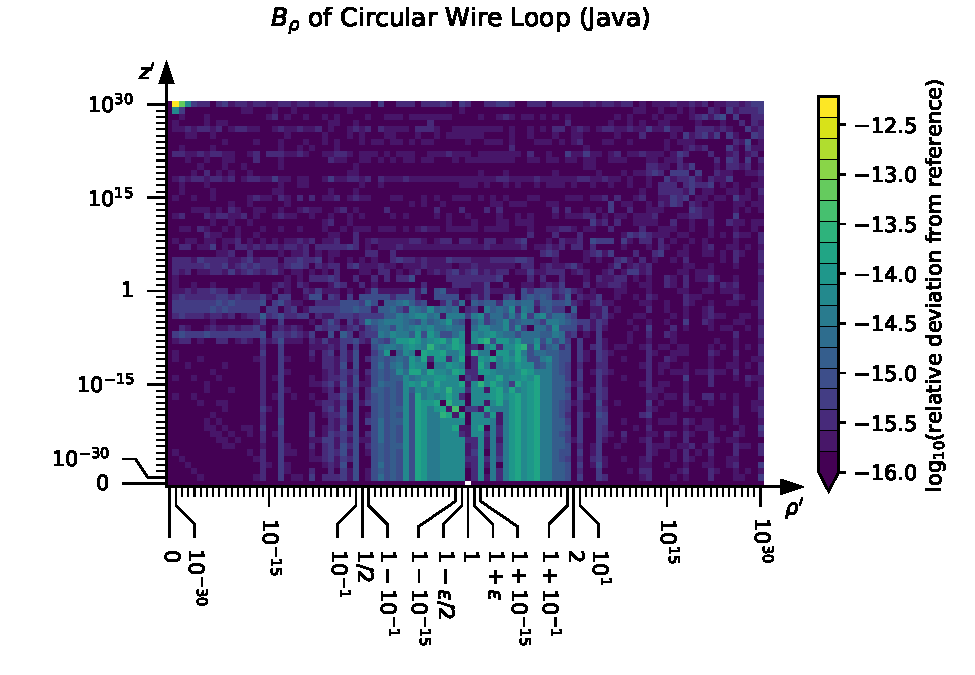
\includegraphics[width=0.8\textwidth]{img/CircularWireLoop_B_rho_Java.pdf}
 \caption{Deviation between Java implementation of \eqn{cwl_B_rho_switchover} and \eqn{B_rho_ref}
          for the computation of $\tilde{B}_\rho$ of a circular wire loop
          in the error metric given by~\eqn{error_metric}.}
 \label{fig:CircularWireLoop_B_rho_Java}
\end{figure}
Fig.~(\ref{fig:CircularWireLoop_B_z_Java}) shows the deviation
according to the error metric~\eqn{error_metric}
between the reference data computed for $\tilde{B}_z$ using \eqn{B_z_ref}
and the results from the \texttt{float64} implementation of \eqn{cwl_B_z_switchover}.
\begin{figure}[htbp]
 \centering
 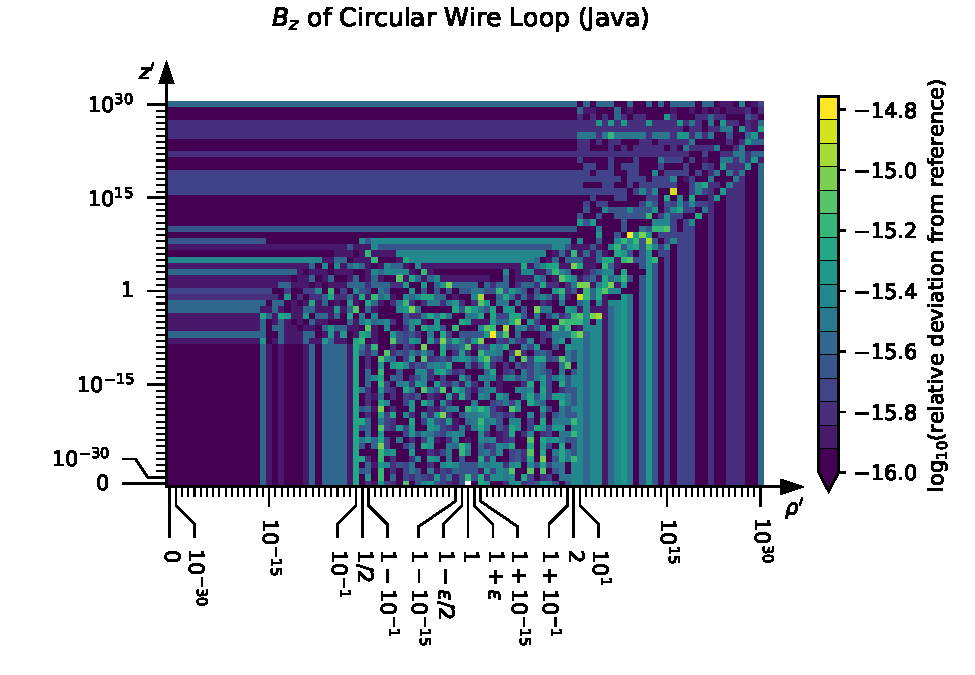
\includegraphics[width=0.8\textwidth]{img/CircularWireLoop_B_z_Java.pdf}
 \caption{Deviation between Java implementation of \eqn{cwl_B_z_switchover} and \eqn{B_z_ref}
          for the computation of $\tilde{B}_z$ of a circular wire loop
          in the error metric given by~\eqn{error_metric}.}
 \label{fig:CircularWireLoop_B_z_Java}
\end{figure}

\FloatBarrier
\subsection{Further tests}
Furthermore, it was tested if the methods presented in this work
can be used to approximate a circular wire loop
by a polygon along the wire down to numerical accuracy.
The geometry of the setup is depicted in Fig.~(\ref{fig:sketch_McGreivy}).
\begin{figure}[htbp]
 \centering
 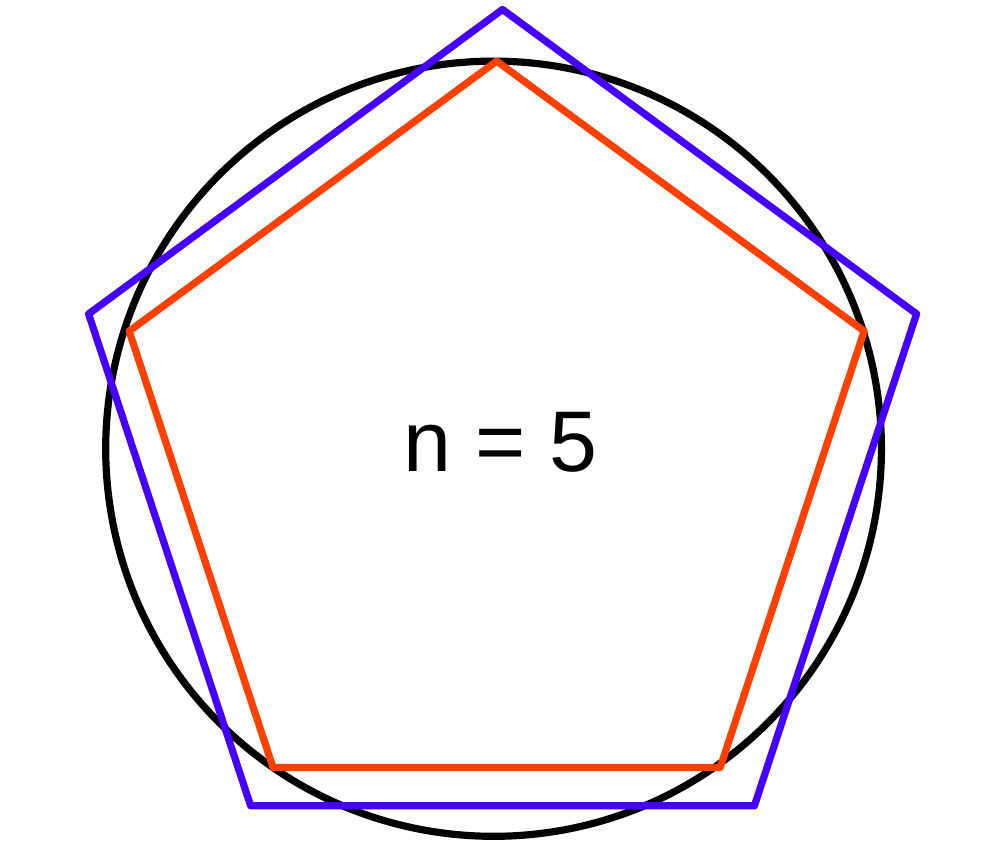
\includegraphics[width=0.4\textwidth]{img/sketch_McGreivy.png}
 \caption{Sketch of the test setup for approximating a circular wire loop by a polygon.
          The current along the wire loop (black) is approximated by
          a current along a polygon with vertices either on the loop (red)
          or vertices adjusted slightly outwards (blue).
          The case of $n=5$ vertices used to approximate the loop is shown here.}
 \label{fig:sketch_McGreivy}
\end{figure}
The expected result is that the relative deviation between
the magnetic field at an arbitrary location
from the circular wire loop and from the corresponding polygon approximation
using straight wire segments vanishes down to numerical accuracy
for a sufficiently large number of points~$n$ used to approximate the wire loop.
A second-order correction to the polygon approximation
for a circular wire loop~\cite{mcgreivy_2021} can be used
to improve the approximation.
Here, the vertices of the polygon used to approximate the wire loop
are adjusted slightly outwards.
Figuratively speaking, in the default case (red polygon in Fig.~\ref{fig:sketch_McGreivy})
the polygon segments are always inside the wire loop
and in the adjusted case (blue polygon in Fig.~\ref{fig:sketch_McGreivy}),
the polygon segments have portions both inside and outside the wire loop.
The results of increasing the number of polygon corners
and observing the decay of the relative error between the analytical wire loop
expression and the approximation by the polygon
are shown in Fig.~(\ref{fig:McGreivy_convergence_2}),
where the orange graph with + symbols (``on-loop'') denotes the case of the polygon vertices on the loop
and the cyan graph with x symbols (``McGreivy'') denotes the case of the polygon vertices adjusted towards the outside
according to Ref.~\cite{mcgreivy_2021}.
In those two cases, standard accumulation using the \texttt{+=} operator
was used to sum up the contributions from the individual wire segments.
It is observed that the results approach numerical accuracy.
but then the error grows again if more polygon vertices are used for the approximation.
This can be explained by considering that the more vertices are used,
the smaller the relative contributions from each individual segment to the total approximation get.
If standard accumulation of the results is used, at some number of polygon corners
it happens that the remaining contributions are getting smaller than the machine precision epsilon
of the current approximation result, thereby effectively ignoring the remaining contributions.
Second-order iterative Kahan-Babuska summation~\cite{klein_2006} had to be used
to circumvent this and achive convergence down to numerical accuracy.
This is shown by the red and blue graphs in Fig.~(\ref{fig:McGreivy_convergence_2}),
where the relative deviation from the reference data does not grow
as the number of polygon corners is increased beyond the threshold for an accurate approximation.
\begin{figure}[htbp]
 \centering
 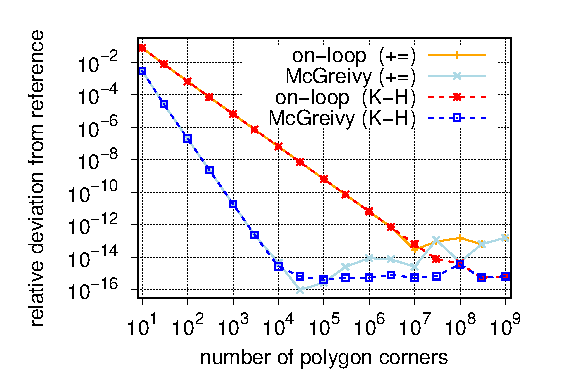
\includegraphics[width=0.8\textwidth]{img/McGreivy_convergence_2.eps}
 \caption{Convergence of the polygon approximation towards the analytical result for the magnetic field of a circular wire loop.
          The vertices of the polygon used to approximate the wire loop have been put on the wire loop (``on-loop'')
          as well as adjusted slightly outwards of the loop according to Ref.~\cite{mcgreivy_2021} (``McGreivy'').
          Standard accumulation using the \texttt{+=} operator (``+='') has been used for the first two graphs (orange and cyan).
          The second two graphs (red and blue) show the results when the accumulation of the individual contributions
          is performed using compensated Kahan-Babushka summation~\cite{klein_2006} (``K-B'')).}
 \label{fig:McGreivy_convergence_2}
\end{figure}








%% The Appendices part is started with the command \appendix;
%% appendix sections are then done as normal sections
\appendix

%% \section{}
%% \label{}

\section{Derivation of General Formulations}
\label{apx:derivation_of_general_formulations}
The derivations of the starting point formulas presented in Sec.~\ref{sec:methods} are given here.

\subsection{Straight Wire Segment}
The following geometric quantities with $\mathbf{x}_f \equiv \mathbf{x}_{i+1}$ are defined to ease the rest of the derivation:
\begin{align}
 L                   & \equiv | \mathbf{x}_f - \mathbf{x}_i | \quad , \\
 \hat{\mathbf{e}}    & \equiv \left(\mathbf{x}_f - \mathbf{x}_i\right) / L \quad , \\
 \mathbf{R}_i        & \equiv \mathbf{x} - \mathbf{x}_i \quad , \\
 \mathbf{R}_f        & \equiv \mathbf{x} - \mathbf{x}_f \quad , \\
 R_i                 & \equiv | \mathbf{R}_i | = | \mathbf{x} - \mathbf{x}_i | \quad , \\
 R_f                 & \equiv | \mathbf{R}_f | = | \mathbf{x} - \mathbf{x}_f | \quad , \\
 R_{i ||}            & \equiv \hat{\mathbf{e}} \cdot \mathbf{R}_i \quad , \\
 R_{f ||}            & \equiv \hat{\mathbf{e}} \cdot \mathbf{R}_f \quad , \\
 \mathbf{R}_\perp    & \equiv \mathbf{R}_i - R_{i ||} \hat{\mathbf{e}} \quad , \\
 R_\perp             & \equiv | \mathbf{R}_\perp | \quad \mathrm{and} \\
 \mathbf{c}(\lambda) & \equiv \mathbf{x}_i + \lambda \left(\mathbf{x}_f - \mathbf{x}_i\right) \quad \mathrm{for} \quad 0 \leq \lambda \leq 1 \quad .
\end{align}
The following relations are also needed:
\begin{align}
       L             & = R_{i ||} - R_{f ||} \\
       R_i^2 - R_f^2 & = L \left( R_{i ||} + R_{f ||} \right) \\
\Rightarrow R_{i ||} & = \frac{R_i^2 - R_f^2}{2 L} + \frac{L}{2} \\
\Rightarrow R_{f ||} & = \frac{R_i^2 - R_f^2}{2 L} - \frac{L}{2}
\end{align}

\subsubsection{Magnetic Vector Potential}
The law of Biot and Savart for the magnetic vector potential of a current density distribution $\mathbf{j}(\mathbf{x})$ is as follows~\cite{jackson}:
\begin{equation}
 \mathbf{A}(\mathbf{x}) = \frac{\mu_0}{4 \pi} \int \frac{\mathbf{j}(\mathbf{x}')}{|\mathbf{x} - \mathbf{x}'|} \mathrm{d}\mathbf{x}' \quad .
\end{equation}
The parametrization of points on the line segment $\mathbf{c}(\lambda)$ can be used to apply this to the given geometry of a wire segment:
\begin{align}
 \mathbf{A}(\mathbf{x}) & = \frac{\mu_0 I}{4 \pi} L \hat{\mathbf{e}} \int\limits_0^1 \frac{\mathrm{d}\lambda}{|\mathbf{x} - \mathbf{c}(\lambda)|} \\
        ~               & = \frac{\mu_0 I}{4 \pi} L \hat{\mathbf{e}} \int\limits_0^1 \frac{\mathrm{d}\lambda}{|\mathbf{x} - \mathbf{x}_i - \lambda L \hat{\mathbf{e}}|} \quad .
\end{align}
A little bit of geometric intuition is needed to simplify the denominator of the integral:
\begin{align}
 \mathbf{x} - \mathbf{x}_i - \lambda L \hat{\mathbf{e}}
   & = \mathbf{R}_i - \lambda L \hat{\mathbf{e}} \\
 ~ & = \mathbf{R}_i - R_{i ||} \hat{\mathbf{e}} + R_{i ||} \hat{\mathbf{e}} - \lambda L \hat{\mathbf{e}} \\
 ~ & = \mathbf{R}_i - R_{i ||} \hat{\mathbf{e}} + \left( R_{i ||} - \lambda L \right) \hat{\mathbf{e}} \\
 ~ & = \mathbf{R}_\perp + \left( R_{i ||} - \lambda L \right) \hat{\mathbf{e}} \quad .
\end{align}
Note that, in particular, $\mathbf{R}_\perp \perp \hat{\mathbf{e}}$ and thus (since $|\hat{\mathbf{e}}|$ = 1) due to Pythagoras:
\begin{equation}
 | \mathbf{x} - \mathbf{x}_i - \lambda L \hat{\mathbf{e}} |^2 = R_\perp^2 + \left( R_{i ||} - \lambda L \right)^2
\end{equation}
and finally with $R_\perp^2 = R_i^2 - R_{i ||}^2$ (also due to Pythagoras):
\begin{align}
 | \mathbf{x} - \mathbf{x}_i - \lambda L \hat{\mathbf{e}} |^2
   & = R_i^2 - R_{i ||}^2 + R_{i ||}^2 - 2 \lambda L R_{i ||} + \lambda^2 L^2 \\
 ~ & = R_i^2 - 2 \lambda L R_{i ||} + \lambda^2 L^2 \quad .
\end{align}
It follows:
\begin{equation}
 \mathbf{A}(\mathbf{x})
 = \frac{\mu_0 I}{4 \pi} L \hat{\mathbf{e}} \int\limits_0^1 \frac{\mathrm{d}\lambda}{\sqrt{R_i^2 - 2 \lambda L R_{i ||} + \lambda^2 L^2}} \quad . \label{eqn:A_integral}
\end{equation}
For $X = a x^2 + b x + c$ with $a>0$ the following relation holds~\cite{bronstein}:
\begin{equation}
 \int \frac{\mathrm{d}x}{\sqrt{X}} = \frac{1}{\sqrt{a}} \log \left( 2 \sqrt{a X} + 2 a x + b \right) \quad .
\end{equation}
Here, $x = \lambda$, $a = L^2$, $b=-2 L R_{i ||}$ and $c=R_i^2$.
The corresponding antiderivative of the integrand in \eqn{A_integral} is:
\begin{equation}
   \int\frac{\mathrm{d}\lambda}{\sqrt{R_i^2 - 2 \lambda L R_{i ||} + \lambda^2 L^2}}
 = \frac{1}{L} \log \left( 2 \sqrt{L^2\left( L^2 \lambda^2 - 2 L R_{i ||} \lambda + R_i^2 \right)} + 2 L^2 \lambda - 2 L R_{i ||} \right) \quad .
\end{equation}
The definite integral in \eqn{A_integral} is therefore solved by the following expression:
\begin{align}
 ~ & \int\limits_0^1 \frac{\mathrm{d}\lambda}{\sqrt{R_i^2 - 2 \lambda L R_{i ||} + \lambda^2 L^2}} \\
 = & \frac{1}{L} \left[ \log \left( 2 \sqrt{L^2\left( L^2 - 2 L R_{i ||} + R_i^2 \right)} + 2 L^2 - 2 L R_{i ||} \right) - \log \left( 2 \sqrt{L^2 R_i^2 } - 2 L R_{i ||} \right) \right] \\
 = & \frac{1}{L} \log \left( \frac{ \bcancel{2 L} \sqrt{L^2 - 2 L R_{i ||} + R_i^2} + \bcancel{2} L^{\bcancel{2}} - \bcancel{2 L} R_{i ||} }{ \bcancel{2 L} R_i - \bcancel{2 L} R_{i ||} } \right)
\end{align}
Note that
\begin{align}
                             L^2 & = L (R_{i ||} - R_{f ||} ) \\
                              ~  & = L R_{i ||} - L R_{f ||} \\
\Rightarrow -2 L R_{i ||} + L^2  & = - \bcancel{2} L R_{i ||}  + \bcancel{L R_{i ||}} - L R_{f ||} \\
                              ~  & = -L (R_{i ||} + R_{f ||} ) \\
                              ~  & = R_f^2 - R_i^2 \\
\Rightarrow                R_f^2 & = R_i^2 -2 L R_{i ||} + L^2 \quad .
\end{align}
Therefore:
\begin{equation}
 \int\limits_0^1 \frac{\mathrm{d}\lambda}{\sqrt{R_i^2 - 2 \lambda L R_{i ||} + \lambda^2 L^2}}
 = \frac{1}{L} \log \left( \frac{ R_f - R_{f ||} }{ R_i - R_{i  \,\mathrm{d}\varphi||} } \right) \quad .
\end{equation}
Inserting this into \eqn{A_integral} leads to the first intermediate result:
\begin{equation}
   \mathbf{A}(\mathbf{x})
 = \frac{\mu_0 I}{4 \pi} \bcancel{L} \bcancel{\frac{1}{L}} \log \left( \frac{ R_f - R_{f ||} }{ R_i - R_{i ||} } \right) \hat{\mathbf{e}}
 = \frac{\mu_0 I}{4 \pi}                                   \log \left( \frac{ R_f - R_{f ||} }{ R_i - R_{i ||} } \right) \hat{\mathbf{e}} \quad . \label{eqn:A_first}
\end{equation}
However, if the point $\mathbf{x}$ is located on the line extension of the wire segment, $R_i = R_{i ||}$ and $R_f = R_{f ||}$,
which leads to a $0/0$ division if this formula is directly evaluated.
The solution is to cancel the singular term $(L + R_f - R_i)$, which is also zero for points on the line extension of the wire segment,
in the numerator and the denominator of \eqn{A_first}.
A second look resolves this:
\begin{align}
\frac{ R_f - R_{f ||} }{ R_i - R_{i ||} }
 = & \frac{ 2 L \left( R_f - R_{f ||} \right) }{ 2 L \left( R_i - R_{i ||} \right) }
 =   \frac{ 2 L R_f - 2 L \left( \frac{R_i^2 - R_f^2}{2 L} - \frac{L}{2} \right) }{ 2 L R_i - 2 L \left( \frac{R_i^2 - R_f^2}{2 L} + \frac{L}{2} \right) } \\
 = & \frac{ 2 L R_f - R_i^2 + R_f^2 + L^2 }{ 2 L R_i - R_i^2 + R_f^2 - L^2 } \\
 = & \frac{ 2 L R_f - R_i^2 + R_f^2 + L^2 + L R_i - L R_i + R_i R_f - R_i R_f}{ 2 L R_i - R_i^2 + R_f^2 - L^2 + L R_f - L R_f + R_i R_f - R_i R_f } \\
 = & \frac{\bcancel{(L + R_f - R_i)}(R_f + R_i + L)}{\bcancel{(L + R_f - R_i)}(R_f + R_i - L)}
 =   \frac{R_f + R_i + L}{R_f + R_i - L} \quad .
\end{align}
It follows for the vector potential expression:
\begin{equation}
 \mathbf{A}(\mathbf{x}) = \frac{\mu_0 I}{4 \pi} \log \left( \frac{R_f + R_i + L}{R_f + R_i - L} \right) \hat{\mathbf{e}} \quad . \label{eqn:A_second}
\end{equation}
The authors of Ref.~\cite{hanson_hirshman_2002} suggest to normalize the length of the wire segment:
\begin{equation}
 \frac{R_f + R_i + L}{R_f + R_i - L} = \frac{1 + \epsilon}{1 - \epsilon} \quad \mathrm{with} ~ \epsilon \equiv \frac{L}{R_i + R_f} \quad ,
\end{equation}
leading to
\begin{equation}
 \mathbf{A}(\mathbf{x}) = \frac{\mu_0 I}{4 \pi} \log\left(\frac{1 + \epsilon}{1 - \epsilon} \right) \hat{\mathbf{e}} \quad . \label{eqn:A_log_eps}
\end{equation}
This is the result for the magnetic vector potential of a filamentary wire segment presented in Ref.~\cite{hanson_hirshman_2002}.
However, for $\epsilon \rightarrow 0$, the numerical evaluation of this expression is problematic.
It is therefore suggested to use the following expression, which works for points extremely close to,
extremely far away from and all in-between locations with respect to the wire segment.
Note that
\begin{equation}
 \mathrm{artanh}\left( \epsilon \right) = \frac{1}{2} \log\left(\frac{1 + \epsilon}{1 - \epsilon} \right) \quad ,
\end{equation}
leading to
\begin{equation}
 \boxed{\mathbf{A}(\mathbf{x}) = \frac{\mu_0 I}{2 \pi} \, \mathrm{artanh} \left( \epsilon \right) \hat{\mathbf{e}}} \quad . \label{eqn:A_artanh}
\end{equation}

\subsubsection{Magnetic Field}
The magnetic field $\mathbf{B}(\mathbf{x})$ is computed from $\mathbf{B} = \nabla \times \mathbf{A}$, applied to \eqn{A_log_eps}.
Define
\begin{equation}
 f(\epsilon) \equiv \log\left(\frac{1 + \epsilon}{1 - \epsilon} \right)
\end{equation}
and it follows:
\begin{equation}
  \frac{4 \pi}{\mu_0 I} \mathbf{B}
 = \nabla \times \left( f(\epsilon) \hat{\mathbf{e}} \right)
 = \nabla f(\epsilon) \times \hat{\mathbf{e}} + f(\epsilon) \underbrace{\nabla \times \hat{\mathbf{e}}}_{=0}
 = f'(\epsilon) \nabla \epsilon \times \hat{\mathbf{e}} \quad .
\end{equation}
Note that
\begin{equation}
   \nabla \epsilon
 = \nabla \left( \frac{L}{R_i + R_f} \right)
 = \frac{-L}{(R_i + R_f)^2}\left( \nabla R_i + \nabla R_f \right)
 = \frac{-L}{(R_i + R_f)^2}\left( \frac{\mathbf{R}_i}{R_i} + \frac{\mathbf{R}_f}{R_f} \right) \quad .
\end{equation}
It follows:
\begin{align}
   \frac{4 \pi}{\mu_0 I} \mathbf{B}
 = & f'(\epsilon) \frac{-L}{(R_i + R_f)^2} \left( \frac{\mathbf{R}_i}{R_i} + \frac{\mathbf{R}_f}{R_f} \right) \times \hat{\mathbf{e}} \\
 = & f'(\epsilon) \frac{L}{(R_i + R_f)^2} \, \hat{\mathbf{e}} \times \left( \frac{\mathbf{R}_i}{R_i} + \frac{\mathbf{R}_f}{R_f} \right) \\
 = & f'(\epsilon) \frac{\epsilon^2}{L}    \, \hat{\mathbf{e}} \times \left( \frac{\mathbf{R}_i}{R_i} + \frac{\mathbf{R}_f}{R_f} \right) \quad . \label{eqn:B_intermediate}
\end{align}
Also:
\begin{align}
   \frac{\mathbf{R}_i}{R_i} + \frac{\mathbf{R}_f}{R_f}
 = & \frac{\mathbf{R}_i}{R_i} + \frac{\mathbf{R}_i - L \hat{\mathbf{e}} }{R_f}
 =   \frac{R_f \mathbf{R}_i + R_i (\mathbf{R}_i - L \hat{\mathbf{e}}) }{R_i R_f}
 =   \frac{(R_f+R_i) \mathbf{R}_i + R_i L \hat{\mathbf{e}} }{R_i R_f} \\
 = & \frac{R_f+R_i}{R_i R_f} \mathbf{R}_i + \frac{R_i L}{R_i R_f} \, \hat{\mathbf{e}}
\end{align}
and therefore:
\begin{equation}
   \hat{\mathbf{e}} \times \left( \frac{\mathbf{R}_i}{R_i} + \frac{\mathbf{R}_f}{R_f} \right)
 = \hat{\mathbf{e}} \times \left( \frac{R_f+R_i}{R_i R_f} \mathbf{R}_i + \frac{R_i L}{R_i R_f} \, \hat{\mathbf{e}} \right)
 = \frac{R_f+R_i}{R_i R_f} \, \hat{\mathbf{e}} \times \mathbf{R}_i \quad ,
\end{equation}
since $\hat{\mathbf{e}} \times \hat{\mathbf{e}} = 0$.
Inserting this into \eqn{B_intermediate} leads to:
\begin{equation}
   \frac{4 \pi}{\mu_0 I} \mathbf{B}
 = f'(\epsilon) \frac{\epsilon^{\bcancel{2}}}{\bcancel{L}} \, \frac{\bcancel{R_f+R_i}}{R_i R_f} \, \hat{\mathbf{e}} \times \mathbf{R}_i
 = f'(\epsilon) \frac{\epsilon}{R_i R_f} \, \hat{\mathbf{e}} \times \mathbf{R}_i \label{eqn:B_intermediate_2}
\end{equation}
Next, look at $f'(\epsilon)$:
\begin{equation}
   f'(\epsilon)
 = \frac{\bcancel{1 - \epsilon}}{1 + \epsilon} \cdot \frac{1 (1-\epsilon) - (1+\epsilon) (-1)}{(1 - \epsilon)^{\bcancel{2}}}
 = \frac{1 - \epsilon + 1 + \epsilon}{(1 + \epsilon)(1 - \epsilon)}
 = \frac{2}{1 - \epsilon^2}
\end{equation}
and insert this into \eqn{B_intermediate_2}:
\begin{align}
   \frac{4 \pi}{\mu_0 I} \mathbf{B}
 = & \frac{2 \epsilon}{1 - \epsilon^2} \cdot \frac{1}{R_i R_f} \, \hat{\mathbf{e}} \times \mathbf{R}_i \\
 = & \frac{2 L}{\bcancel{R_i + R_f}} \cdot \frac{(R_i + R_f)^{\bcancel{2}}}{(R_i + R_f)^2 - L^2} \cdot \frac{1}{R_i R_f} \, \hat{\mathbf{e}} \times \mathbf{R}_i \quad .
\end{align}
This results in the final expression for the magnetic field:
\begin{equation}
 \boxed{\mathbf{B} (\mathbf{x}) = \frac{\mu_0 I}{4 \pi} \frac{2 L (R_i + R_f)}{R_i R_f} \frac{1}{(R_i + R_f)^2 - L^2} \, \hat{\mathbf{e}} \times \mathbf{R}_i } \quad .
\end{equation}

\subsection{Circular Wire Loop}
The current density of the wire loop can be expressed as follows:
\begin{equation}
  \mathbf{j}(\mathbf{x}') = I \delta(\rho' - a) \delta(z') \,\hat{\mathbf{e}}_{\varphi'} \, .
\end{equation}

\subsubsection{Magnetic Vector Potential}
The Biot-Savart law for the magnetic vector potential reads:
\begin{align}
  \mathbf{A}(\mathbf{x}) &= \frac{\mu_0  }{4 \pi}
                            \int_{\realnumbers^3}
                              \frac{\mathbf{j}(\mathbf{x}')}{|\mathbf{x} - \mathbf{x}'|} \,\mathrm{d}^3\mathbf{x}' \nonumber \\
             ~           &= \frac{\mu_0 I}{4 \pi}
                            \int_{\realnumbers^3}
                              \frac{\delta(\rho' - a) \delta(z')}{|\mathbf{x} - \mathbf{x}'|} \,\hat{\mathbf{e}}_{\varphi'}
                              \,\mathrm{d}^3\mathbf{x}' \nonumber \\
             ~           &= \frac{\mu_0 I}{4 \pi}
                            \int\limits_{-\infty}^{\infty} \int\limits_{0}^{2 \pi} \int\limits_{0}^{\infty}
                              \frac{\delta(\rho' - a) \delta(z')}{|\mathbf{x} - \mathbf{x}'|} \,\hat{\mathbf{e}}_{\varphi'}
                              \rho' \,\mathrm{d} \rho' \,\mathrm{d} \varphi'  \,\mathrm{d} z' \label{eqn:vecpot_loop_general}
\end{align}
where a change of variables from Cartesian coordinates to cylindrical coordinates was performed in the integral.
The differential volume element was adjusted according to
$\,\mathrm{d}^3\mathbf{x}' = \rho' \,\mathrm{d} \rho' \,\mathrm{d} \varphi'  \,\mathrm{d} z'$.
The coordinate system is rotated around the $z$ axis to yield $\varphi=0$ for the evaluation location $\mathbf{x}$
which is generally acceptable due to the rotational symmetry of the circular wire loop.
Then, $\mathbf{x} = (x, y, z)$ in Cartesian coordinates with
\begin{align}
  x &= \rho \cos(\varphi) = \rho \\
  y &= \rho \sin(\varphi) = 0    \, .
\end{align}
The distance $|\mathbf{x} - \mathbf{x}'|$ is then:
\begin{align}
  |\mathbf{x} - \mathbf{x}'| &= \sqrt{(\rho - \rho' \cos(\varphi'))^2 + \rho'^2 \sin^2(\varphi') + (z - z')^2} \nonumber \\
              ~              &= \sqrt{ \rho^2 + \rho'^2 (\cos(\varphi'))^2 + \sin^2(\varphi')) - 2 \rho \rho' \cos(\varphi') + (z - z')^2} \nonumber \\
              ~              &= \sqrt{ \rho^2 + \rho'^2 + (z - z')^2 - 2 \rho \rho' \cos(\varphi')} \, .
\end{align}
Inserting this into \eqn{vecpot_loop_general} leads to:
\begin{equation}
  \mathbf{A}(\mathbf{x}) = \frac{\mu_0 I}{4 \pi} \int\limits_{-\infty}^{\infty} \int\limits_{0}^{2 \pi} \int\limits_{0}^{\infty}
                                                             \frac{\delta(\rho' - a) \delta(z')}{\sqrt{ \rho^2 + \rho'^2 + (z - z')^2 - 2 \rho \rho' \cos(\varphi')}}
                                                             \,\hat{\mathbf{e}}_{\varphi'}
                                                             \rho' \,\mathrm{d} \rho' \,\mathrm{d} \varphi'  \,\mathrm{d} z'
\end{equation}
and the integrals over $\rho'$ and $z'$ can be evaluated already:
\begin{equation}
  \mathbf{A}(\mathbf{x}) = \frac{\mu_0 I a}{4 \pi}
                           \int\limits_{0}^{2 \pi}
                             \frac{\hat{\mathbf{e}}_{\varphi'} \,\mathrm{d} \varphi'}{\sqrt{ \rho^2 + a^2 + z^2 - 2 \rho a \cos(\varphi')}} \, . \label{eqn:vecpot_loop_phiprime}
\end{equation}
The cylindrical components of the magnetic vector potential~$\mathbf{A}$ are obtained
by dotting above result with the cylindrical unit vector at the evaluation location~$\mathbf{x}$:
\begin{equation}
  \mathbf{A}(\mathbf{x}) =   A_\rho    \,\hat{\mathbf{e}}_\rho
                           + A_\varphi \,\hat{\mathbf{e}}_\varphi
                           + A_z       \,\hat{\mathbf{e}}_z
\end{equation}
with
\begin{align}
  A_\rho    &= \mathbf{A}(\mathbf{x}) \cdot \,\hat{\mathbf{e}}_\rho    \\
  A_\varphi &= \mathbf{A}(\mathbf{x}) \cdot \,\hat{\mathbf{e}}_\varphi \\
  A_z       &= \mathbf{A}(\mathbf{x}) \cdot \,\hat{\mathbf{e}}_z       \, .
\end{align}
The dot products of the cylindrical unit vectors are:
\begin{align}
  \hat{\mathbf{e}}_{\varphi'} \cdot \,\hat{\mathbf{e}}_\rho    &= \begin{pmatrix} -\sin(\varphi') \\ \cos(\varphi') \\ 0 \end{pmatrix}
                                                                  \cdot
                                                                  \begin{pmatrix}  \cos(\varphi ) \\ \sin(\varphi ) \\ 0 \end{pmatrix}
                                                                = \begin{pmatrix} -\sin(\varphi') \\ \cos(\varphi') \\ 0 \end{pmatrix}
                                                                  \cdot
                                                                  \begin{pmatrix}  1 \\ 0 \\ 0 \end{pmatrix}
                                                                = -\sin(\varphi') \\
  \hat{\mathbf{e}}_{\varphi'} \cdot \,\hat{\mathbf{e}}_\varphi &= \begin{pmatrix} -\sin(\varphi') \\ \cos(\varphi') \\ 0 \end{pmatrix}
                                                                  \cdot
                                                                  \begin{pmatrix} -\sin(\varphi ) \\ \cos(\varphi ) \\ 0 \end{pmatrix}
                                                                = \begin{pmatrix} -\sin(\varphi') \\ \cos(\varphi') \\ 0 \end{pmatrix}
                                                                  \cdot
                                                                  \begin{pmatrix}  0 \\ 1 \\ 0 \end{pmatrix}
                                                                =  \cos(\varphi') \\
  \hat{\mathbf{e}}_{\varphi'} \cdot \,\hat{\mathbf{e}}_z       &= \begin{pmatrix} -\sin(\varphi') \\ \cos(\varphi') \\ 0 \end{pmatrix}
                                                                  \cdot
                                                                  \begin{pmatrix} 0 \\ 0 \\ 1 \end{pmatrix}
                                                                = 0 \, . \label{eqn:e_phiprime_dot_ez}
\end{align}
The expression from \eqn{vecpot_loop_phiprime} is inserted into above expressions.
The vertical component~$A_z$ vanishes trivially since the unit vectors are orthogonal,
as can be seen from \eqn{e_phiprime_dot_ez}.
For the radial component $A_\rho$ it follows:
\begin{equation}
  A_\rho = \frac{\mu_0 I a}{4 \pi}
           \int\limits_{0}^{2 \pi}
             \frac{-\sin(\varphi') \,\mathrm{d} \varphi'}{\sqrt{ \rho^2 + a^2 + z^2 - 2 \rho a \cos(\varphi')}} = 0 \, ,
\end{equation}
since the integrand is an odd function of $\varphi'$.
The tangential component $A_\varphi$ is non-zero because the integrand is an even function of $\varphi'$.
It is given by:
\begin{equation}
  A_\varphi(\rho, z) = \frac{\mu_0 I a}{4 \pi}
                       \int\limits_{0}^{2 \pi}
                         \frac{\cos(\varphi') \,\mathrm{d} \varphi'}{\sqrt{ \rho^2 + a^2 + z^2 - 2 \rho a \cos(\varphi')}} \, , \label{eqn:a_phi_general}
\end{equation}
leading to
\begin{equation}
  \mathbf{A}(\mathbf{x}) = A_\varphi(\rho, z) \,\hat{\mathbf{e}}_\varphi \, . \label{eqn:a_cwl_components}
\end{equation}
A change of variables from $\varphi'$ to $\beta$ is performed in order to solve \eqn{a_phi_general}:
\begin{equation}
 \varphi' = 2 \beta + \pi
\end{equation}
which implies
\begin{align}
 \frac{\mathrm{d}\varphi'}{\mathrm{d}\beta} = 2     &\Rightarrow \mathrm{d}\varphi' = 2 \mathrm{d}\beta \\
                                 \varphi'_0 = 0     &\Rightarrow           \beta_0 = - \frac{\pi}{2}   \\
                                 \varphi'_1 = 2 \pi &\Rightarrow           \beta_1 =   \frac{\pi}{2}   \, .
\end{align}
It follows for \eqn{a_phi_general}:
\begin{equation}
 A_\varphi(\rho, z) = \frac{\mu_0 I a}{4 \pi}
                       \int\limits_{-\pi/2}^{\pi/2}
                         \frac{2 \cos(2 \beta + \pi) \,\mathrm{d}\beta}
                              {\sqrt{\rho^2 + a^2 + z^2 - 2 \rho a \cos(2 \beta + \pi)}} \, .
\end{equation}
Note that $\cos(2 \beta + \pi) = - \cos(2 \beta)$:
\begin{equation}
 A_\varphi(\rho, z) = \frac{\mu_0 I a}{2 \pi}
                       \int\limits_{-\pi/2}^{\pi/2}
                         \frac{-\cos(2 \beta) \,\mathrm{d}\beta}
                              {\sqrt{\rho^2 + a^2 + z^2 + 2 \rho a \cos(2 \beta)}} \, . \label{eqn:a_phi_progress}
\end{equation}
In the numerator of the integrand it follows:
\begin{equation}
 -\cos(2 \beta) = -\left(\cos^2(\beta) - \sin^2(\beta) \right) = \sin^2(\beta) - \cos^2(\beta) \, .
\end{equation}
The denominator of the integrand can be reformulated by introducing normalized coordinates
$\rho' = \rho/a$ and $z' = z/a$ as follows:
\begin{align}
 ~ & \rho^2 + a^2 + z^2 + 2 \rho a \cos(2 \beta) \nonumber \\
 ~ &= a^2 \left[z'^2 +      \rho'^2 + 1        + 2 \rho' \cos(2 \beta)         \right] \nonumber \\
 ~ &= a^2 \left[z'^2 + (1 + \rho')^2 - 2 \rho' + 2 \rho' \cos(2 \beta)         \right] \nonumber \\
 ~ &= a^2 \left[z'^2 + (1 + \rho')^2 - 2 \rho' \left(1 - \cos(2 \beta) \right) \right] \nonumber \\
 ~ &= a^2 \left[z'^2 + (1 + \rho')^2 - 2 \rho' \left(1 + \sin^2(\beta) - \cos^2(\beta) \right) \right] \nonumber \\
 ~ &= a^2 \left[z'^2 + (1 + \rho')^2 - 2 \rho' \left(\bcancel{\cos^2(\beta)} + \sin^2(\beta) + \sin^2(\beta) \bcancel{- \cos^2(\beta)} \right) \right] \nonumber \\
 ~ &= a^2 \left[z'^2 + (1 + \rho')^2 - 4 \rho' \sin^2(\beta) \right] \nonumber \\
 ~ &= a^2 \left( z'^2 + (1 + \rho')^2 \right) \Biggl[1 - \underbrace{\frac{4 \rho'}{z'^2 + (1 + \rho')^2}}_{\equiv k^2} \sin^2(\beta) \Biggr] \nonumber \\
 ~ &= a^2 \left( z'^2 + (1 + \rho')^2 \right) \left [1 - k^2 \sin^2(\beta) \right] \label{eqn:a_phi_denom_refactor_start}
\end{align}
with
\begin{equation}
 k^2 = \frac{4 \rho'}{z'^2 + (1 + \rho')^2} \, . \label{eqn:my_k_sq}
\end{equation}
Inserting this into \eqn{a_phi_progress} leads to:
\begin{equation}
 A_\varphi(\rho', z') = \frac{\mu_0 I}
                           {2 \pi}
                      \frac{1}
                           {\sqrt{z'^2 + (1 + \rho')^2}}
                      \int\limits_{-\pi/2}^{\pi/2}
                        \frac{\sin^2(\beta) - \cos^2(\beta)}
                             {\sqrt{1 - k^2 \sin^2(\beta)}}
                        \,\mathrm{d}\beta \, .
\end{equation}
Focusing again on the denominator of the integrand:
\begin{align}
 1 - k^2 \sin^2(\beta)
   &= \cos^2(\beta) + \sin^2(\beta) - \frac{4 \rho'}{z'^2 + (1 + \rho')^2} \sin^2(\beta) \nonumber \\
 ~ &= \cos^2(\beta) + \left(1 - \frac{4 \rho'}{z'^2 + (1 + \rho')^2}\right) \sin^2(\beta) \nonumber \\
 ~ &= \cos^2(\beta) + \frac{z'^2 + (1 + \rho')^2 - 4 \rho'}{z'^2 + (1 + \rho')^2} \sin^2(\beta) \nonumber \\
 ~ &= \cos^2(\beta) + \underbrace{\frac{z'^2 + (1 - \rho')^2}{z'^2 + (1 + \rho')^2}}_{\equiv k_c^2} \sin^2(\beta) \nonumber \\
 ~ &= \cos^2(\beta) + k_c^2 \sin^2(\beta) \label{eqn:a_phi_denom_refactor_done}
\end{align}
with
\begin{equation}
 k_c^2 = \frac{z'^2 + (1 - \rho')^2}{z'^2 + (1 + \rho')^2} \, , \label{eqn:k_c_final}
\end{equation}
leading to:
\begin{equation}
 A_\varphi(\rho', z') = \frac{\mu_0 I}
                           {2 \pi}
                      \frac{1}
                           {\sqrt{z'^2 + (1 + \rho')^2}}
                      \int\limits_{-\pi/2}^{\pi/2}
                        \frac{\sin^2(\beta) - \cos^2(\beta)}
                             {\sqrt{\cos^2(\beta) + k_c^2 \sin^2(\beta)}}
                        \,\mathrm{d}\beta \, .
\end{equation}
The integrand is symmetric about $0$ and therefore the integration domain can be halved if a factor of $2$ is included:
\begin{equation}
 A_\varphi(\rho', z') = \frac{\mu_0 I}
                           {\pi}
                      \frac{1}
                           {\sqrt{z'^2 + (1 + \rho')^2}}
                      \int\limits_{0}^{\pi/2}
                        \frac{\sin^2(\beta) - \cos^2(\beta)}
                             {\sqrt{\cos^2(\beta) + k_c^2 \sin^2(\beta)}}
                        \,\mathrm{d}\beta \, .
\end{equation}
The remaining integral is a complete elliptic integral which can be expressed using the form
introduced by Bulirsch~\cite{bulirsch_3}:
\begin{equation}
  \mathrm{cel}(k_c, p, a, b)
= \int\limits_{0}^{\pi/2}
   \frac{a \cos^2(\varphi) + b \sin^2(\varphi)}
        {  \cos^2(\varphi) + p \sin^2(\varphi)}
   \frac{\mathrm{d}\varphi}
        {\sqrt{\cos^2(\varphi) + k_\mathrm{c}^2 \sin^2(\varphi)}} \, .
\end{equation}
Note that the parameter $a$ of $\mathrm{cel}(k_c, p, a, b)$ is not to be confused with the radius of the wire loop.
A numerical implementation of the general complete elliptic integral $\mathrm{cel}(k_c, p, a, b)$ is provided in the cited article.
The use of this particular implementation is inspired by Ref.~\cite{teal}.
Putting above results together, we arrive at the following expression for $A_\varphi$:
\begin{equation}
 \boxed{A_\varphi(\rho', z') = \frac{\mu_0 I}{\pi}
                               \frac{1}{\sqrt{z'^2 + (1 + \rho')^2}}
                               \,\mathrm{cel}(k_c, 1, -1, 1)} \, . \label{eqn:A_phi_final}
\end{equation}
In Eqn.~(5.37) of Ref.~\cite{jackson} the tangential component is given by:
\begin{align}
  A_\varphi(r, \theta) &= \frac{\mu_0}{4 \pi}
                          \frac{4 I a}{\sqrt{a^2 + r^2 + 2 a r \sin(\theta)}}
                          \left[
                            \frac{(2 - k^2)K(k) - 2 E(k)}{k^2}
                          \right] \label{eqn:aphi_initial}
\end{align}
with
\begin{equation}
  k^2 = \frac{4 a r \sin(\theta)}{a^2 + r^2 + 2 a r \sin(\theta)} \, .
\end{equation}
Here, $K(k)$ and $E(k)$ are the complete elliptic integrals of the first and second kind, respectively.
Spherical coordinates are used with $r \sin(\theta) = \rho$ and $r^2 = \rho^2 + z^2$.
In order to bring this to the form in \eqn{A_phi_final},
an expression for the linear combination of $K(k)$ and $E(k)$ from Ref.~\cite{bulirsch_3} is used:
\begin{equation}
  \lambda K(k) + \mu E(k) = \,\mathrm{cel}(k_c, 1, \lambda + \mu, \lambda + \mu k_c^2)
\end{equation}
where
\begin{equation}
  k^2 + k_\mathrm{c}^2 = 1 \, .
\end{equation}
The argument of the elliptic integrals is considered first:
\begin{align}
  k^2 &= \frac{4 a r \sin(\theta)}{a^2 + r^2 + 2 a r \sin(\theta)}
       = \frac{4 a \rho}{a^2 + r^2 + 2 a \rho}
       = \frac{4 \bcancel{a} \rho}{a^{\bcancel{2}} \left(1 + \frac{r^2}{a^2} + 2 \frac{\rho}{a} \right)} \nonumber \\
  ~   &= \frac{4 \rho'}{1 + \frac{r^2}{a^2} + 2 \rho'}
       = 4 \rho' \left( 1 + \frac{\rho^2 + z^2}{a^2} + 2 \rho' \right)^{-1}
       = 4 \rho' \left( 1 + \rho'^{2} + z'^{2} + 2 \rho' \right)^{-1} \nonumber \\
  ~   &= \frac{4 \rho'}{z'^2 + (1 + \rho')^2} \, .
\end{align}
Thus, $k^2$ from Ref.~\cite{jackson} is equivalent to $k^2$ in \eqn{my_k_sq}.
Inserting this into \eqn{aphi_initial} leads to:
\begin{align}
  A_\varphi(r, \theta) &= \frac{\mu_0 I}{\bcancel{2} \pi}
                          \frac{\bcancel{2}}{\sqrt{z'^2 + (1 + \rho')^2}}
                          \left[
                            \frac{(2 - k^2)K(k) - 2 E(k)}{k^2}
                          \right] \nonumber \\
           ~           &= \frac{\mu_0 I}{\pi}
                          \frac{1}{\sqrt{z'^2 + (1 + \rho')^2}}
                          \left[
                            \frac{(2 - k^2)K(k) - 2 E(k)}{k^2}
                          \right] \, .
\end{align}
The coefficients of the elliptic integrals are given as follows:
\begin{align}
  \lambda &= \frac{2 - k^2}{k^2} = \frac{2}{k^2} - 1 \\
  \mu     &= -\frac{2}{k^2}
\end{align}
and their combinations are as follows:
\begin{align}
  \lambda + \mu       &= \frac{2}{k^2} - 1 - \frac{2}{k^2}     = -1 \\
  \lambda + \mu k_c^2 &= \frac{2}{k^2} - 1 - \frac{2}{k^2} (1 - k^2) \nonumber \\
          ~           &= \frac{2}{k^2} - 1 - \frac{2}{k^2} + 2 =  1 \, .
\end{align}
Putting above results together, we arrive at the following expression for $A_\varphi$:
\begin{equation}
 \boxed{A_\varphi(r, \theta) = \frac{\mu_0 I}{\pi}
                            \frac{1}{\sqrt{z'^2 + (1 + \rho')^2}} \,\mathrm{cel}(k_c, 1, -1, 1)}
\end{equation}
with $\rho' = r/a \sin(\theta)$, $z' = \sqrt{r^2 - \rho^2}/a$ and $k_c$ given by \eqn{k_c_final}).
It is favorable for numerical evaluation of $A_\varphi$ to use the form given in \eqn{A_phi_final}
where the linear combination of the complete elliptic integrals is embedded in the parameters of $\mathrm{cel}(k_c, p, a, b)$
and no precautions need to be taken to deal with cancellations in \eqn{aphi_initial}.

\subsubsection{Magnetic Field}
The magnetic field is computed using $\mathbf{B} = \nabla \times \mathbf{A}$.
In cylindrical coordinates with the form of the magnetic vector potential from \eqn{a_cwl_components}
the curl is given as follows:
\begin{equation}
  \mathbf{B}(\mathbf{x})
= B_\rho \hat{\mathbf{e}}_\rho + B_z \hat{\mathbf{e}}_z
\end{equation}
with
\begin{align}
  B_\rho &= -                \frac{\partial       A_\varphi }{\partial z   }  \label{eqn:b_rho_start} \\
  B_z    &=   \frac{1}{\rho} \frac{\partial (\rho A_\varphi)}{\partial \rho}
          = \frac{A_\varphi}{\rho} + \frac{\partial A_\varphi}{\partial \rho} \label{eqn:b_z_start} \, .
\end{align}
Starting from \eqn{a_phi_general} it is noted that the partial derivatives only act on the denominator of the integrand.
Therefore, consider first:
\begin{align}
  \frac{\partial}{\partial z} \left( a^2 + z^2 + \rho^2 - 2 a \rho \cos(\varphi) \right)^{-\frac{1}{2}}
  ~ &= - \bcancel{\frac{1}{2}} \left( a^2 + z^2 + \rho^2 - 2 a \rho \cos(\varphi) \right)^{-\frac{3}{2}} \left( \bcancel{2} z \right) \nonumber \\
  ~ &= \frac{- z}{\left[ a^2 + z^2 + \rho^2 - 2 a \rho \cos(\varphi) \right]^{\frac{3}{2}}} \\
  \frac{\partial}{\partial \rho} \left( a^2 + z^2 + \rho^2 - 2 a \rho \cos(\varphi) \right)^{-\frac{1}{2}}
  ~ &= - \bcancel{\frac{1}{2}} \left( a^2 + z^2 + \rho^2 - 2 a \rho \cos(\varphi) \right)^{-\frac{3}{2}} \left( \bcancel{2} \rho - \bcancel{2} a \cos(\varphi) \right) \nonumber \\
  ~ &= \frac{-(\rho - a \cos(\varphi))}{\left[ a^2 + z^2 + \rho^2 - 2 a \rho \cos(\varphi) \right]^{\frac{3}{2}}} \, .
\end{align}
These expressions are used to formulate \eqn{b_rho_start} and
a change of variables from $\varphi$ to $\beta$ analogously to the step from \eqn{a_phi_general} to \eqn{a_phi_progress} is performed.
Finally, normalized coordinates are introduced in the integrand similar to the steps from \eqn{a_phi_denom_refactor_start} to \eqn{a_phi_denom_refactor_done}:
\begin{align}
  B_\rho &= \frac{\partial}{\partial z} \left(
             \frac{\mu_0 I a}{4 \pi}
             \int\limits_{0}^{2 \pi}
               \frac{\cos(\varphi') \,\mathrm{d} \varphi'}{\sqrt{ \rho^2 + a^2 + z^2 - 2 \rho a \cos(\varphi')}} \right) \nonumber \\
    ~    &= - \frac{\mu_0 I a z}{4 \pi}
              \int\limits_{0}^{2 \pi}
                \frac{\cos(\varphi') \,\mathrm{d} \varphi'}
                     {\left[a^2 + z^2 + \rho^2 - 2 a \rho \cos(\varphi') \right]^{\frac{3}{2}}} \nonumber \\
    ~    &=   \frac{\mu_0 I a z}{2 \pi}
              \int\limits_{-\pi/2}^{\pi/2}
                \frac{\cos(2 \beta) \,\mathrm{d}\beta}
                     {\left[a^2 + z^2 + \rho^2 + 2 a \rho \cos(2 \beta) \right]^{\frac{3}{2}}} \nonumber \\
     ~    &=  \frac{\mu_0 I}{2 \pi}
              \frac{\cancel{a^2} z'}{a^{\bcancel{3}} \left( z'^2 + (1 + \rho')^2 \right)^{\frac{3}{2}}}
              \int\limits_{-\pi/2}^{\pi/2}
                \frac{\sin^2(\beta) - \cos^2(\beta)}
                     { \left[\cos^2(\beta) + k_c^2 \sin^2(\beta) \right]^{\frac{3}{2}} }
                \,\mathrm{d}\beta \label{eqn:B_rho_almost}
\end{align}
This integrand is also symmetric about $0$, which can be used to express \eqn{B_rho_almost} in terms of the general complete elliptic integral:
\begin{equation}
  \boxed{B_\rho(\rho', z') =
    \frac{\mu_0 I}{\pi a}
    \frac{z'}{\left[ z'^2 + (1 + \rho')^2 \right]^{\frac{3}{2}}}
    \,\mathrm{cel}(k_c, k_c^2, -1, 1) } \, . \label{eqn:B_rho_final}
\end{equation}
Regarding $B_z$ the first term in \eqn{b_z_start} can already be written down using $\rho = a \rho'$ and $A_\varphi$ from \eqn{A_phi_final}:
\begin{equation}
  B_z = \frac{\mu_0 I}{\pi a}
        \frac{1}{\rho' \sqrt{z'^2 + (1 + \rho')^2}}
        \,\mathrm{cel}(k_c, 1, -1, 1)
        + \frac{\partial A_\varphi}{\partial \rho} \label{eqn:B_z_intermediate}
\end{equation}
The second term is considered next:
\begin{align}
      \frac{\partial A_\varphi}{\partial \rho}
 =&\, \frac{\partial A_\varphi}{\partial \rho'} \frac{\partial \rho'}{\partial \rho}
 =    \frac{1}{a} \frac{\partial A_\varphi}{\partial \rho'} \nonumber \\
 =&\, \frac{1}{a} \frac{\partial}{\partial \rho'} \left[
                               \frac{\mu_0 I}{\pi}
                               \frac{1}{\sqrt{z'^2 + (1 + \rho')^2}}
                               \,\mathrm{cel}(k_c, 1, -1, 1) \right] \nonumber \\
 =&\, \frac{\mu_0 I}{\pi a} \frac{\partial}{\partial \rho'} \left[
        \frac{1}{\sqrt{z'^2 + (1 + \rho')^2}} \,\mathrm{cel}(k_c, 1, -1, 1) \right] \nonumber \\
 =&\,          \frac{\mu_0 I}{\pi a} \Biggl\{ \phantom{+}
        \frac{\partial}{\partial \rho'} \left[ \frac{1}{\sqrt{z'^2 + (1 + \rho')^2}} \right] \,\mathrm{cel}(k_c, 1, -1, 1) \nonumber \\
 ~&\, \phantom{\frac{\mu_0 I}{\pi a} \Biggl\{}         +
        \frac{1}{\sqrt{z'^2 + (1 + \rho')^2}} \frac{\partial}{\partial \rho'} \,\mathrm{cel}(k_c, 1, -1, 1) \Biggr\} \nonumber \\
 =&\,          \frac{\mu_0 I}{\pi a} \Biggl\{ \phantom{+}
        \frac{-(1+\rho')}{\left[z'^2 + (1 + \rho')^2\right]^{3/2}}\,\mathrm{cel}(k_c, 1, -1, 1) \nonumber \\
 ~&\, \phantom{\frac{\mu_0 I}{\pi a} \Biggl\{}         +
        \frac{1}{\sqrt{z'^2 + (1 + \rho')^2}} \frac{\partial (k_c^2)}{\partial \rho'}
        \frac{\partial}{\partial (k_c^2)} \,\mathrm{cel}(k_c, 1, -1, 1)\, \Biggr\} \label{eqn:dAphiDrho} \, .
\end{align}
Consider the remaining derivatives:
\begin{align}
      \frac{\partial (k_c^2)}{\partial \rho'}
 =&\, \frac{\partial}{\partial \rho'} \left( \frac{z'^2 + (1 - \rho')^2}{z'^2 + (1 + \rho')^2} \right) \nonumber \\
 =&\, \frac{1}{z'^2 + (1 + \rho')^2} \left(-2(1 - \rho') - k_c^2 \, 2 (1 + \rho') \right) \nonumber \\
 =&\, \frac{-2}{z'^2 + (1 + \rho')^2} \left(1 - \rho' + k_c^2 (1 + \rho') \right) \nonumber \\
 =&\, \frac{-2}{z'^2 + (1 + \rho')^2} \left(1 + k_c^2 - (1 - k_c^2) \rho' \right)
\end{align}
as well as:
\begin{align}
 \frac{\partial}{\partial (k_c^2)}& \,\mathrm{cel}(k_c, 1, -1, 1) \nonumber \\
 =&\, \frac{\partial}{\partial (k_c^2)} \int\limits_0^{\pi/2} \frac{\sin^2(\varphi) - \cos^2(\varphi)}
                                                                   {\sqrt{\cos^2(\varphi) + k_c^2 \sin^2(\varphi)}} \,\mathrm{d}\varphi \nonumber \\
 =&\, \int\limits_0^{\pi/2} \left[ \sin^2(\varphi) - \cos^2(\varphi) \right]
        \frac{\partial}{\partial (k_c^2)} \left[ \cos^2(\varphi) + k_c^2 \sin^2(\varphi) \right]^{-1/2} \,\mathrm{d}\varphi \nonumber \\
 =&\, \int\limits_0^{\pi/2} \left[ \sin^2(\varphi) - \cos^2(\varphi) \right]
        \left(-\frac{1}{2}\right) \left[ \cos^2(\varphi) + k_c^2 \sin^2(\varphi) \right]^{-3/2} \sin^2(\varphi) \,\mathrm{d}\varphi \nonumber \\
 =&\, -\frac{1}{2} \int\limits_0^{\pi/2} \frac{\left[\sin^2(\varphi) - \cos^2(\varphi) \right] \sin^2(\varphi)}
                                              {\left[\cos^2(\varphi) + k_c^2 \sin^2(\varphi) \right]^{3/2}}  \,\mathrm{d}\varphi \, .
\end{align}
These terms are now inserted into \eqn{dAphiDrho}:
\begin{align}
      \frac{\partial A_\varphi}{\partial \rho}
 =&\, \frac{\mu_0 I}{\pi a} \Biggl\{ \phantom{+}
        \frac{-(1+\rho')}{\left[z'^2 + (1 + \rho')^2\right]^{3/2}} \,\mathrm{cel}(k_c, 1, -1, 1) \nonumber \\
 ~&\, \phantom{\frac{\mu_0 I}{\pi a} \Biggl\{}         +
        \frac{1}{\sqrt{z'^2 + (1 + \rho')^2}}
        \frac{\bcancel{-2}}{z'^2 + (1 + \rho')^2} \left(1 + k_c^2 - (1 - k_c^2) \rho' \right) \nonumber \\
 ~&\, \phantom{\frac{\mu_0 I}{\pi a} \Biggl\{ +}
        \bcancel{\left(-\frac{1}{2} \right)}
        \int\limits_0^{\pi/2}
          \frac{\left[\sin^2(\varphi) - \cos^2(\varphi) \right] \sin^2(\varphi)}
               {\left[\cos^2(\varphi) + k_c^2 \sin^2(\varphi) \right]^{3/2}}  \,\mathrm{d}\varphi \, \Biggr\} \nonumber \\
 =&\, \frac{\mu_0 I}{\pi a} \Biggl\{
      \phantom{+}\,
      \frac{-(1 + \rho')}{\left[z'^2 + (1 + \rho')^2\right]^{3/2}}
      \,\mathrm{cel}(k_c, 1, -1, 1) \nonumber \\
 ~&\, \phantom{\frac{\mu_0 I}{\pi a} \Biggl\{}
      + \frac{1 + k_c^2 - (1 - k_c^2) \rho'}{\left[z'^2 + (1 + \rho')^2\right]^{3/2}}
        \int\limits_0^{\pi/2}
          \frac{\left[\sin^2(\varphi) - \cos^2(\varphi) \right] \sin^2(\varphi)}
               {\left[\cos^2(\varphi) + k_c^2 \sin^2(\varphi) \right]^{3/2}}  \,\mathrm{d}\varphi \Biggr\} \, .
\end{align}
This form of $\partial A_\varphi / \partial \rho$ is now inserted into \eqn{B_z_intermediate}.
$\partial A_\varphi / \partial \rho$ has to be multiplied by a factor of $\rho'$ in order to factor out a common prefactor $1/\rho'$.
This leads to:
\begin{align}
  B_z
 =&\, \frac{\mu_0 I}{\pi a}
      \frac{1}{\rho' \sqrt{z'^2 + (1 + \rho')^2}} \Biggl\{ \,\mathrm{cel}(k_c, 1, -1, 1) - \frac{\rho' (1+\rho')}{z'^2 + (1 + \rho')^2} \,\mathrm{cel}(k_c, 1, -1, 1) \nonumber \\
 ~&\, + \frac{\rho' \left[1 + k_c^2 - (1 - k_c^2) \rho'\right]}{z'^2 + (1 + \rho')^2}
          \int\limits_0^{\pi/2}
          \frac{\left[\sin^2(\varphi) - \cos^2(\varphi) \right] \sin^2(\varphi)}
               {\left[\cos^2(\varphi) + k_c^2 \sin^2(\varphi) \right]^{3/2}}  \,\mathrm{d}\varphi \Biggr\} \nonumber \\
 =&\, \frac{\mu_0 I}{\pi a}
      \frac{1}{\rho' \sqrt{z'^2 + (1 + \rho')^2}} \Biggl\{ \left( 1 - \frac{\rho' (1+\rho')}{z'^2 + (1 + \rho')^2}\right) \,\mathrm{cel}(k_c, 1, -1, 1) \nonumber \\
 ~&\, + \frac{\rho' \left[1 + k_c^2 - (1 - k_c^2) \rho'\right]}{z'^2 + (1 + \rho')^2}
          \int\limits_0^{\pi/2}
          \frac{\left[\sin^2(\varphi) - \cos^2(\varphi) \right] \sin^2(\varphi)}
               {\left[\cos^2(\varphi) + k_c^2 \sin^2(\varphi) \right]^{3/2}}  \,\mathrm{d}\varphi \Biggr\} \nonumber \\
 =&\, \frac{\mu_0 I}{\pi a}
      \frac{1}{\rho' \sqrt{z'^2 + (1 + \rho')^2}} \Biggl\{ \left( 1 - \frac{\rho' (1+\rho')}{z'^2 + (1 + \rho')^2}\right)
      \int\limits_0^{\pi/2}
        \frac{\sin^2(\varphi) - \cos^2(\varphi)}
             {\sqrt{\cos^2(\varphi) + k_c^2 \sin^2(\varphi)}} \,\mathrm{d}\varphi \nonumber \\
 ~&\, + \frac{\rho' \left[1 + k_c^2 - (1 - k_c^2) \rho'\right]}{z'^2 + (1 + \rho')^2}
          \int\limits_0^{\pi/2}
          \frac{\left[\sin^2(\varphi) - \cos^2(\varphi) \right] \sin^2(\varphi)}
               {\left[\cos^2(\varphi) + k_c^2 \sin^2(\varphi) \right]^{3/2}}  \,\mathrm{d}\varphi \Biggr\} \, .
\end{align}
The integrand of the two integrals can be combined.
A nutritious one needs to be included in the first integrand:
\begin{align}
  B_z
 =&\, \frac{\mu_0 I}{\pi a}
      \frac{1}{\rho' \sqrt{z'^2 + (1 + \rho')^2}}
      \int\limits_0^{\pi/2} \,\mathrm{d}\varphi\,
        \frac{\sin^2(\varphi) - \cos^2(\varphi)}
             {\left[\cos^2(\varphi) + k_c^2 \sin^2(\varphi) \right]^{3/2}} \nonumber \\
 \Biggl\{ &\left( 1 - \frac{\rho' (1+\rho')}{z'^2 + (1 + \rho')^2} \right)
            \left[ \cos^2(\varphi) + k_c^2 \sin^2(\varphi) \right]
          + \frac{\rho' \left[1 + k_c^2 - (1 - k_c^2) \rho'\right]}{z'^2 + (1 + \rho')^2} \sin^2(\varphi)
        \Biggr\} \, .
\end{align}
Consider for now only the part inside the $\{\}$ of above equation:
\begin{align}
 ~&\,   \left( 1 - \frac{\rho' (1+\rho')}{z'^2 + (1 + \rho')^2} \right)
        \left[ \cos^2(\varphi) + k_c^2 \sin^2(\varphi) \right]
      + \frac{\rho' \left[1 + k_c^2 - (1 - k_c^2) \rho'\right]}{z'^2 + (1 + \rho')^2} \sin^2(\varphi) \nonumber \\
 =&\, \frac{1}{z'^2 + (1 + \rho')^2} \Biggl\{
        \left[ z'^2 + (1 + \rho')^2 - \rho' (1+\rho') \right] \left[ \cos^2(\varphi) + k_c^2 \sin^2(\varphi) \right] \nonumber \\
 ~&\, \phantom{\frac{1}{z'^2 + (1 + \rho')^2} \Biggl\{}
      + \rho' \left[1 + k_c^2 - (1 - k_c^2) \rho'\right] \sin^2(\varphi) \Biggr\}
\end{align}
and in there also only the part inside the $\{\}$:
\begin{align}
 ~&\, \left[ z'^2 + (1 + \rho')^2 - \rho' (1+\rho') \right] \left[ \cos^2(\varphi) + k_c^2 \sin^2(\varphi) \right] \nonumber \\
 ~&\, + \rho' \left[1 + k_c^2 - (1 - k_c^2) \rho'\right] \sin^2(\varphi) \nonumber \\
 =&\, \left[ z'^2 + (1 + \rho')^2 - \rho' (1+\rho') \right] \left[ \cos^2(\varphi) + \frac{z'^2 + (1 - \rho')^2}{z'^2 + (1 + \rho')^2} \sin^2(\varphi) \right] \nonumber \\
 ~&\, + \rho' \left[1 + k_c^2 - (1 - k_c^2) \rho'\right] \sin^2(\varphi) \nonumber \\
 =&\, \left[ z'^2 + (1 + \rho')^2 \right] \cos^2(\varphi) + \left[ z'^2 + (1 - \rho')^2 \right] \sin^2(\varphi)                                        & \Bigr\} \equiv (*)~\, \nonumber \\
 ~&\, - \rho' (1+\rho') \left[ \cos^2(\varphi) + k_c^2 \sin^2(\varphi) \right] + \rho' \left[1 + k_c^2 - (1 - k_c^2) \rho'\right] \sin^2(\varphi) \, . & \Bigr\} \equiv (**) \label{eqn:starStar}
\end{align}
The two contributions are simplified separately:
\begin{align}
 (*)
 =&\, \left[ z'^2 + 1 + 2 \rho' + \rho'^2 \right] \cos^2(\varphi) + \left[ z'^2 + 1 - 2 \rho' + \rho'^2  \right] \sin^2(\varphi) \nonumber \\
 =&\, z'^2 + 1 + \rho'^2 + 2 \rho' \left[ \cos^2(\varphi) - \sin^2(\varphi) \right]
\end{align}
as well as:
\begin{align}
  (**)
 =&\, - \rho' \cos^2(\varphi) - \rho'^2 \cos^2(\varphi) \cancel{- \rho' k_c^2 \sin^2(\varphi)}                           \bcancel{- \rho'^2 k_c^2 \sin^2(\varphi)} \nonumber \\
 ~&\, + \rho' \sin^2(\varphi)                           \cancel{+ \rho' k_c^2 \sin^2(\varphi)} - \rho'^2 \sin^2(\varphi) \bcancel{+ \rho'^2 k_c^2 \sin^2(\varphi)} \nonumber \\
 =&\, - \rho' \left[ \cos^2(\varphi) - \sin^2(\varphi) \right] - \rho'^2 \underbrace{\left[ \cos^2(\varphi) + \sin^2(\varphi) \right]}_{=1}
\end{align}
Combining them to form \eqn{starStar} leads to:
\begin{align}
  (*) + (**)
 =&\, z'^2 + 1 \bcancel{+ \rho'^2} + \cancel{2} \rho' \left[ \cos^2(\varphi) - \sin^2(\varphi) \right] \cancel{- \rho' \left[ \cos^2(\varphi) - \sin^2(\varphi) \right]} \bcancel{- \rho'^2} \nonumber \\
 =&\, z'^2 + 1 + \rho' \left[ \cos^2(\varphi) - \sin^2(\varphi) \right] \, .
\end{align}
The full form of $B_z$ is assembled again now based on the recent findings to remind ourselves of the state of things:
\begin{align}
 B_z
 =&\, \frac{\mu_0 I}{\pi a}
      \frac{1}{\rho' \sqrt{z'^2 + (1 + \rho')^2}} \nonumber \\
 ~&\, \int\limits_0^{\pi/2}
        \frac{\sin^2(\varphi) - \cos^2(\varphi)}
             {\left[\cos^2(\varphi) + k_c^2 \sin^2(\varphi) \right]^{3/2}}
        \frac{1}{z'^2 + (1 + \rho')^2}
        \left\{ z'^2 + 1 + \rho' \left[ \cos^2(\varphi) - \sin^2(\varphi) \right] \right\} \,\mathrm{d}\varphi \, . \label{eqn:B_z_core}
\end{align}
The term in $\{\}$ in above integrand is now restructured :
\begin{align}
 ~&\, z'^2 + 1 + \rho' \left[ \cos^2(\varphi) - \sin^2(\varphi) \right] \nonumber \\
 =&\, \frac{1}{2} z'^2 + \frac{1}{2} \left( z'^2 + 1 - \rho'^2 \right) + \frac{1}{2} \left\{ 1 + \rho'^2 + 2 \rho' \left[ \cos^2(\varphi) - \sin^2(\varphi) \right] \right\} \nonumber \\
 =&\, \phantom{+}~
        \frac{1}{2} z'^2 \left[ \cos^2(\varphi) + \sin^2(\varphi) \right]
      + \frac{1}{2} \left( z'^2 + 1 - \rho'^2 \right) \nonumber \\
 ~&\, + \frac{1}{2} \Bigl[   \underbrace{\left( 1 + 2 \rho' + \rho'^2 \right)}_{=(1+\rho')^2} \cos^2(\varphi)
                           + \underbrace{\left( 1 - 2 \rho' + \rho'^2 \right)}_{=(1-\rho')^2} \sin^2(\varphi) \Bigr] \nonumber \\
 =&\,   \frac{1}{2} \left[ z'^2 + (1 + \rho')^2 \right] \cos^2(\varphi) + \frac{1}{2} \left[ z'^2 + (1 - \rho')^2 \right] \sin^2(\varphi)
      + \underbrace{\frac{1}{2} \left( z'^2 + 1 + \rho'^2 \right)}_{(*)} \underbrace{- \rho'^2}_{(**)} \label{eqn:bZCore} \, .
\end{align}
Consider $(*)$ and $(**)$ separately:
\begin{align}
 (*)
 =&\, \frac{1}{2} z'^2 + \frac{1}{4} \Bigl[ \underbrace{1 + 2 \rho' + \rho'^2}_{=(1+\rho')^2} + \underbrace{1 - 2 \rho' + \rho'^2}_{=(1-\rho')^2} \Bigr] \nonumber \\
 =&\, \frac{1}{4} \left[ z'^2 + (1 + \rho')^2 + z^2 + (1 - \rho')^2 \right] \nonumber \\
 =&\, \frac{1}{4} \left[ z'^2 + (1 + \rho')^2 \right] + \frac{1}{4} \left[ z^2 + (1 - \rho')^2 \right]
\end{align}
and
\begin{align}
  (**)
 =&\, \frac{1}{4} \rho' \left[ z'^2 + 1 - 2 \rho' + \rho'^2 - \left( z'^2 + 1 + 2 \rho' + \rho'^2 \right) \right] \nonumber \\
 =&\, \frac{1}{4} \rho' \left[ z'^2 + ( 1 - \rho')^2 \right] - \frac{1}{4} \rho' \left[ z'^2 + (1 + \rho')^2 \right] \, .
\end{align}
These expressions are now inserted into \eqn{bZCore}, leading to:
\begin{align}
 ~&\, \phantom{+}~
        \frac{1}{2} \left[ z'^2 + (1 + \rho')^2 \right] \cos^2(\varphi) + \frac{1}{2} \left[ z'^2 + (1 - \rho')^2 \right] \sin^2(\varphi) \nonumber \\
 ~&\, + \frac{1}{4} \left[ z'^2 + (1 + \rho')^2 \right] + \frac{1}{4} \left[ z^2 + (1 - \rho')^2 \right] \nonumber \\
 ~&\, + \frac{1}{4} \rho' \left[ z'^2 + ( 1 - \rho')^2 \right] - \frac{1}{4} \rho' \left[ z'^2 + (1 + \rho')^2 \right] \nonumber \\
 =&\, \left[ z'^2 + (1 + \rho')^2 \right] \Biggl\{
        \frac{1}{2} \cos^2(\varphi) + \underbrace{\frac{z'^2 + (1 - \rho')^2}{z'^2 + (1 + \rho')^2}}_{=k_c^2} \sin^2(\varphi) \nonumber \\
 ~&\, \phantom{\left[ z'^2 + (1 + \rho')^2 \right] \Biggl\{}
        + \frac{1}{4} \Biggl[ 1 + \underbrace{\frac{z'^2 + (1 - \rho')^2}{z'^2 + (1 + \rho')^2}}_{=k_c^2}
                              - \Biggl( 1 - \underbrace{\frac{z'^2 + (1 - \rho')^2}{z'^2 + (1 + \rho')^2}}_{=k_c^2} \Biggr) \rho' \Biggr] \Biggr\} \nonumber \\
 =&\, \left[ z'^2 + (1 + \rho')^2 \right] \left\{
          \frac{1}{2} \left[ \cos^2(\varphi) + k_c^2 \sin^2(\varphi) \right]
        + \frac{1}{4} \left[ 1 + k_c^2 - \left( 1 - k_c^2 \right) \rho' \right] \right\} \, .
\end{align}
This is now inserted back into \eqn{B_z_core}:
\begin{align}
  B_z
 =&\, \frac{\mu_0 I}{\pi a}
      \frac{1}{\rho' \sqrt{z'^2 + (1 + \rho')^2}}
      \int\limits_0^{\pi/2}
        \frac{\sin^2(\varphi) - \cos^2(\varphi)}
             {\left[\cos^2(\varphi) + k_c^2 \sin^2(\varphi) \right]^{3/2}} \nonumber \\
 ~&\,   \left\{   \frac{1}{2} \left[ \cos^2(\varphi) + k_c^2 \sin^2(\varphi) \right]
                + \frac{1}{4} \left[ 1 + k_c^2 - \left( 1 - k_c^2 \right) \rho' \right] \right\} \,\mathrm{d}\varphi \, .
\end{align}
The integral can be split up back again into two integrals:
\begin{align}
  B_z
 =&\, \frac{\mu_0 I}{\pi a}
      \frac{1}{\rho' \sqrt{z'^2 + (1 + \rho')^2}} \Biggl[
        \frac{1}{2} \underbrace{\int\limits_0^{\pi/2} \frac{\sin^2(\varphi) - \cos^2(\varphi)}
                                                           {\sqrt{\cos^2(\varphi) + k_c^2 \sin^2(\varphi)}} \,\mathrm{d}\varphi}_{=\textrm{cel}(k_c, 1, -1, 1)} \nonumber \\
 ~&\, + \frac{1}{4} \left[ 1 + k_c^2 - \left( 1 - k_c^2 \right) \rho' \right]
          \underbrace{\int\limits_0^{\pi/2} \frac{\sin^2(\varphi) - \cos^2(\varphi)}
                                                 {\left[\cos^2(\varphi) + k_c^2 \sin^2(\varphi) \right]^{3/2}} \,\mathrm{d}\varphi}_{=\textrm{cel}(k_c, k_c^2, -1, 1)} \Biggr] \, .
\end{align}
This concludes the derivation of the expression for $B_z$ of a circular wire loop
and here is the final result as published in Ref.~\cite{teal}:
\begin{equation}
\boxed{
 B_z(\rho', z')
 = \frac{\mu_0 I}{2 \pi a}
   \frac{1}{\rho' \sqrt{z'^2 + (1 + \rho')^2}}
   \left[
       \textrm{cel}(k_c, 1, -1, 1)
     + \frac{1 + k_c^2 - \left( 1 - k_c^2 \right) \rho'}{2} \textrm{cel}(k_c, k_c^2, -1, 1)
   \right]
}
\end{equation}

\section{Derivation of Special Case Formulations}
\label{apx:derivation_of_special_case_formulations}



%% References
%%
%% Following citation commands can be used in the body text:
%% Usage of \cite is as follows:
%%   \cite{key}         ==>>  [#]
%%   \cite[chap. 2]{key} ==>> [#, chap. 2]
%%

%% References with bibTeX database:

\bibliographystyle{elsarticle-num}
\bibliography{bibliography.bib}

%% Authors are advised to submit their bibtex database files. They are
%% requested to list a bibtex style file in the manuscript if they do
%% not want to use elsarticle-num.bst.

%% References without bibTeX database:

% \begin{thebibliography}{00}

%% \bibitem must have the following form:
%%   \bibitem{key}...
%%

% \bibitem{}

% \end{thebibliography}


\end{document}

%%
%% End of file
